%╔════════════════════════════╗
%║	  Szablon dostosował	  ║
%║	mgr inż. Dawid Kotlarski  ║
%║		  08.10.2022		  ║
%╚════════════════════════════╝
\documentclass[12pt,twoside,a4paper,openany]{article}

    % ------------------------------------------------------------------------
% PAKIETY
% ------------------------------------------------------------------------

%różne pakiety matematyczne, warto przejrzeć dokumentację, muszą być powyżej ustawień językowych.
\usepackage{mathrsfs}   %Różne symbole matematyczne opisane w katalogu ~\doc\latex\comprehensive. Zamienia \mathcal{L} ze zwykłego L na L-transformatę.
\usepackage{eucal}      %Różne symbole matematyczne.
\usepackage{amssymb}    %Różne symbole matematyczne.
\usepackage{amsmath}    %Dodatkowe funkcje matematyczne, np. polecenie \dfac{}{} skladajace ulamek w trybie wystawionym (porównaj $\dfrac{1}{2}$, a $\frac{1}{2}$).

%język polski i klawiatura
\usepackage[polish]{babel}
%\usepackage{qtimes} % czcionka Times new Roman
\usepackage[OT4]{polski}
%\usepackage[cp1250]{inputenc}                       %Strona kodowa polskich znaków.

%obsługa pdf'a
\usepackage[pdftex,usenames,dvipsnames]{color}      %Obsługa kolorów. Opcje usenames i dvipsnames wprowadzają dodatkowe nazwy kolorow.
\usepackage[pdftex,pagebackref=false,draft=false,pdfpagelabels=false,colorlinks=true,urlcolor=blue,linkcolor=black,citecolor=green,pdfstartview=FitH,pdfstartpage=1,pdfpagemode=UseOutlines,bookmarks=true,bookmarksopen=true,bookmarksopenlevel=2,bookmarksnumbered=true,pdfauthor={Dawid Kotlarski},pdftitle={Praca Inznierska},pdfsubject={},pdfkeywords={transient recovery voltage trv},unicode=true]{hyperref}   %Opcja pagebackref=true dotyczy bibliografii: pokazuje w spisie literatury numery stron, na których odwołano się do danej pozycji.

%bibliografia
%\usepackage[numbers,sort&compress]{natbib}  %Porządkuje zawartość odnośników do literatury, np. [2-4,6]. Musi być pod pdf'em, a styl bibliogfafii musi mieć nazwę z dodatkiem 'nat', np. \bibliographystyle{unsrtnat} (w kolejności cytowania).
\usepackage[
backend=biber,
style=numeric,
sorting=none
]{biblatex}
\addbibresource{bibliografia.bib}
\usepackage{hypernat}                       %Potrzebna pakietowi natbib do wspolpracy z pakietem hyperref (wazna kolejnosc: 1. hyperref, 2. natbib, 3. hypernat).

%grafika i geometria strony
\usepackage{extsizes}           %Dostepne inne rozmiary czcionek, np. 14 w poleceniu: \documentclass[14pt]{article}.
\usepackage[final]{graphicx}
\usepackage[a4paper,left=3.5cm,right=2.5cm,top=2.5cm,bottom=2.5cm]{geometry}

%strona tytułowa
\usepackage{strona_tytulowa}

%inne
\usepackage[hide]{todo}                     %Wprowadza polecenie \todo{treść}. Opcje pakietu: hide/show. Polecenie \todos ma byc na koncu dokumentu, wszystkie \todo{} po \todos sa ignorowane.
\usepackage[basic,physics]{circ}            %Wprowadza środowisko circuit do rysowania obwodów elektrycznych. Musi byc poniżej pakietow językowych.
\usepackage[sf,bf,outermarks]{titlesec}     %Troszczy się o wygląd tytułów rozdziałów (section, subsection, ...). sf oznacza czcionkę sans serif (typu arial), bf -- bold. U mnie: oddzielna linia dla naglowku paragraph. Patrz tez: tocloft -- lepiej robi format spisu tresci.
\usepackage{tocloft}                        %Troszczy się o format spisu trsci.
\usepackage{expdlist}    %Zmienia definicję środowiska description, daje większe możliwości wpływu na wygląd listy.
\usepackage{flafter}     %Wprowadza parametr [tb] do polecenia \suppressfloats[t] (polecenie to powoduje nie umieszczanie rysunkow, tabel itp. na stronach, na ktorych jest to polecenie (np. moze byc to stroma z tytulem rozdzialu, ktory chcemy zeby byl u samej gory, a nie np. pod rysunkiem)).
\usepackage{array}       %Ładniej drukuje tabelki (np. daje wiecej miejsca w komorkach -- nie są tak ścieśnione, jak bez tego pakietu).
\usepackage{listings}    %Listingi programow.
\usepackage[format=hang,labelsep=period,labelfont={bf,small},textfont=small]{caption}   %Formatuje podpisy pod rysunkami i tabelami. Parametr 'hang' powoduje wcięcie kolejnych linii podpisu na szerokosc nazwy podpisu, np. 'Rysunek 1.'.
\usepackage{appendix}    %Troszczy się o załączniki.
\usepackage{floatflt}    %Troszczy się o oblewanie rysunkow tekstem.
\usepackage{here}        %Wprowadza dodtkowy parametr umiejscowienia rysunków, tabel, itp.: H (duże). Umiejscawia obiekty ruchome dokladnie tam gdzie są w kodzie źródłowym dokumentu.
\usepackage{makeidx}     %Troszczy się o indeks (skorowidz).

%nieużywane, ale potencjalnie przydatne
\usepackage{sectsty}           %Formatuje nagłówki, np. żeby były kolorowe -- polecenie: \allsectionsfont{\color{Blue}}.
%\usepackage{version}           %Wersje dokumentu.

%============
\usepackage{longtable}			%tabelka
%============

%============
% Ustawienia listingów do kodu
%============

\usepackage{listings}
\usepackage{xcolor}

\definecolor{codegreen}{rgb}{0,0.6,0}
\definecolor{codegray}{rgb}{0.5,0.5,0.5}
\definecolor{codepurple}{rgb}{0.58,0,0.82}
\definecolor{backcolour}{rgb}{0.95,0.95,0.92}

% Definicja stylu "mystyle"
\lstdefinestyle{mystyle}{
	backgroundcolor=\color{backcolour},   
	commentstyle=\color{codegreen},
	keywordstyle=\color{blue},	%magenta
	numberstyle=\tiny\color{codegray},
	stringstyle=\color{codepurple},
	basicstyle=\ttfamily\footnotesize,
	breakatwhitespace=false,         
	breaklines=true,                 
	captionpos=b,                    
	keepspaces=true,                 
	numbers=left,                    
	numbersep=5pt,                  
	showspaces=false,                
	showstringspaces=false,
	showtabs=false,                  
	tabsize=2
}

\lstset{style=mystyle} % Deklaracja aktywnego stylu
%===========

%PAGINA GÓRNA I DOLNA
\usepackage{fancyhdr}          %Dodaje naglowki jakie się chce.
\pagestyle{fancy}
\fancyhf{}
% numery stron w paginie dolnej na srodku
\fancyfoot[C]{\scriptsize DOKUMENTACJA PROJEKTU - PROGRAMOWANIE URZĄDZEŃ MOBILNCH \\ 
\normalsize\sffamily  \thepage}


%\fancyhead[L]{\small\sffamily \nouppercase{\leftmark}}
\fancyhead[C]{\footnotesize \textit{AKADEMIA NAUK STOSOWANYCH W NOWYM SĄCZU}\\}

\renewcommand{\headrulewidth}{0.4pt}
\renewcommand{\footrulewidth}{0.4pt}

    % ------------------------------------------------------------------------
% USTAWIENIA
% ------------------------------------------------------------------------

% ------------------------------------------------------------------------
%   Kropki po numerach sekcji, podsekcji, itd.
%   Np. 1.2. Tytuł podrozdziału
% ------------------------------------------------------------------------
\makeatletter
    \def\numberline#1{\hb@xt@\@tempdima{#1.\hfil}}                      %kropki w spisie treści
    \renewcommand*\@seccntformat[1]{\csname the#1\endcsname.\enspace}   %kropki w treści dokumentu
\makeatother

% ------------------------------------------------------------------------
%   Numeracja równań, rysunków i tabel
%   Np.: (1.2), gdzie:
%   1 - numer sekcji, 2 - numer równania, rysunku, tabeli
%   Uwaga ogólna: o otoczeniu figure ma być najpierw \caption{}, potem \label{}, inaczej odnośnik nie działa!
% ------------------------------------------------------------------------
\makeatletter
    \@addtoreset{equation}{section} %resetuje licznik po rozpoczęciu nowej sekcji
    \renewcommand{\theequation}{{\thesection}.\@arabic\c@equation} %dodaje kropki

    \@addtoreset{figure}{section}
    \renewcommand{\thefigure}{{\thesection}.\@arabic\c@figure}

    \@addtoreset{table}{section}
    \renewcommand{\thetable}{{\thesection}.\@arabic\c@table}
\makeatother

% ------------------------------------------------------------------------
% Tablica
% ------------------------------------------------------------------------
\newenvironment{tabela}[3]
{
    \begin{table}[!htb]
    \centering
    \caption[#1]{#2}
    \vskip 9pt
    #3
}{
    \end{table}
}

% ------------------------------------------------------------------------
% Dostosowanie wyglądu pozycji listy \todos, np. zamiast 'p.' jest 'str.'
% ------------------------------------------------------------------------
\renewcommand{\todoitem}[2]{%
    \item \label{todo:\thetodo}%
    \ifx#1\todomark%
        \else\textbf{#1 }%
    \fi%
    (str.~\pageref{todopage:\thetodo})\ #2}
\renewcommand{\todoname}{Do zrobienia...}
\renewcommand{\todomark}{~uzupełnić}

% ------------------------------------------------------------------------
% Definicje
% ------------------------------------------------------------------------
\def\nonumsection#1{%
    \section*{#1}%
    \addcontentsline{toc}{section}{#1}%
    }
\def\nonumsubsection#1{%
    \subsection*{#1}%
    \addcontentsline{toc}{subsection}{#1}%
    }
\reversemarginpar %umieszcza notki po lewej stronie, czyli tam gdzie jest więcej miejsca
\def\notka#1{%
    \marginpar{\footnotesize{#1}}%
    }
\def\mathcal#1{%
    \mathscr{#1}%
    }
\newcommand{\atp}{ATP/EMTP} % Inaczej: \def\atp{ATP/EMTP}

% ------------------------------------------------------------------------
% Inne
% ------------------------------------------------------------------------
\frenchspacing                      
\hyphenation{ATP/-EMTP}             %dzielenie wyrazu w danym miejscu
\setlength{\parskip}{3pt}           %odstęp pomiędzy akapitami
\linespread{1.3}                    %odstęp pomiędzy liniami (interlinia)
\setcounter{tocdepth}{4}            %uwzględnianie w spisie treści czterech poziomów sekcji
\setcounter{secnumdepth}{4}         %numerowanie do czwartego poziomu sekcji 
\titleformat{\paragraph}[hang]      %wygląd nagłówków
{\normalfont\sffamily\bfseries}{\theparagraph}{1em}{}



    %polecenia zdefiniowane w pakiecie strona_tytulowa.sty
    \title{Operatsiya 'Kooperatsiya'(Operacja kooperacja)}		%...Wpisać nazwę projektu...
    \author{Maciej Śmierciak}
    \authorI{Michał Jonak}
    \authorII{Konrad Szczurek}		%jeśli są dwie osoby w projekcie to zostawiamy:    \authorII{}
		
	\uczelnia{AKADEMIA NAUK STOSOWANYCH \\W NOWYM SĄCZU}
    \instytut{Wydział Nauk Inżynieryjnych}
    \kierunek{Katedra Informatyki}
    \praca{DOKUMENTACJA PROJEKTOWA}
    \przedmiot{PROGRAMOWANIE URZĄDZEŃ MOBILNYCH}
    \prowadzacy{mgr inż. Dawid Kotlarski}
    \rok{2022}


%definicja składni mikrotik
\usepackage{fancyvrb}
\DefineVerbatimEnvironment{MT}{Verbatim}%
{commandchars=\+\[\],fontsize=\small,formatcom=\color{red},frame=lines,baselinestretch=1,} 
\let\mt\verb 
%zakonczenie definicji składni mikrotik

\usepackage{fancyhdr}    %biblioteka do nagłówka i stopki

			
\begin{document}
   
    \renewcommand{\figurename}{Rys.}    %musi byc pod \begin{document}, bo w~tym miejscu pakiet 'babel' narzuca swoje ustawienia
    \renewcommand{\tablename}{Tab.}     %j.w.
    \thispagestyle{empty}               %na tej stronie: brak numeru
    \stronatytulowa                     %strona tytułowa tworzona przez pakiet strona_tytulowa.tex
 
 \pagestyle{fancy}

    \newpage

    %formatowanie spisu treści i~nagłówków
    \renewcommand{\cftbeforesecskip}{8pt}
    \renewcommand{\cftsecafterpnum}{\vskip 8pt}
    \renewcommand{\cftparskip}{3pt}
    \renewcommand{\cfttoctitlefont}{\Large\bfseries\sffamily}
    \renewcommand{\cftsecfont}{\bfseries\sffamily}
    \renewcommand{\cftsubsecfont}{\sffamily}
    \renewcommand{\cftsubsubsecfont}{\sffamily}
    \renewcommand{\cftparafont}{\sffamily}
    %koniec formatowania spisu treści i nagłówków
     
    \tableofcontents    %spis treści
    \thispagestyle{fancy}
    \newpage

    
    \newpage

    
%%%%%%%%%%%%%%%%%%% treść główna dokumentu %%%%%%%%%%%%%%%%%%%%%%%%%

   	\newpage
\section{Ogólne określenie wymagań}		%1
%Ogólne określenie wymagań i zakresu programu (Czyli zleceniodawca określa wymagania programu) 















\subsection{Gra logiczna}  %1.1       

Projektem jest gra logiczna możliwa do zagrania tylko w trybie kooperacji. Gra będzie opierać się na stosunkowo łatwych zagadkach, które będzie można rozwiązać tylko współpracując.
\\Ogólnym konceptem jest podzielenie gry na 2 główne części:
\\\hspace{0.60cm}-Tryb graficzny,
\\\hspace{0.60cm}-Tryb tekstowy.


%
%rysunek

	\begin{figure}[!htb]
	\begin{center}
		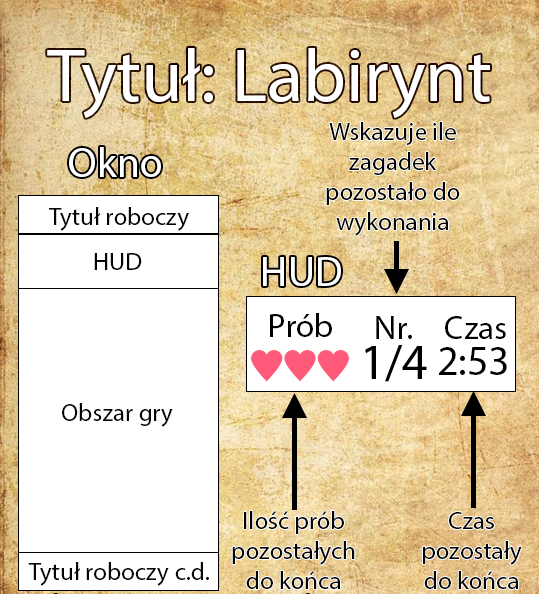
\includegraphics[width=8cm]{rys/gra1.png}
		\caption{Labirynt}
		\label{rys:rysunek001}
	\end{center}
\end{figure}

\hspace{-0.60cm}Jak możemy zauważyć na rysunku 1.1 będziemy mieli określoną liczbę żyć na rozwiązanie określonej liczby zagadek w określonym czasie. W tym trybie zagadki będą polegały na wyjściu z labiryntu.
\\
\\
\\
\\
\\
\\
\\
\\
	\begin{figure}[!htb]
	\begin{center}
		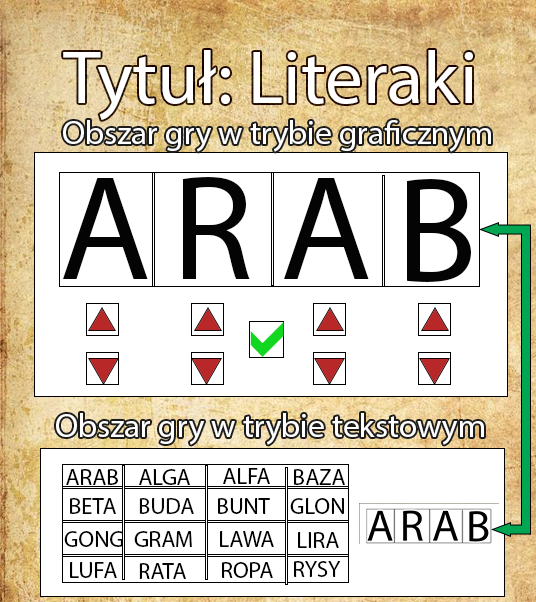
\includegraphics[width=8cm]{rys/gra4.png}
		\caption{Literaki}
		\label{rys:rysunek001}
	\end{center}
\end{figure}

\hspace{-0.60cm}W trybie gry Literaki gracze mają za zadanie ułożyć czteroliterowy wyraz, który nakłada się z wyrazem w bazie. Dostęp do bazy wyrazów ma gracz w trybie tekstowym. Gracz obsługujący tryb graficzny za pomocą strzałek zmienia litery na danej pozycji. 
\\Ze względu na to, ze nie wszystkie litery są na wszystkich polach możliwość będzie tylko jedna. Błędna kombinacja oznacza utratę jednego z żyć. Podobnie jak w trybie labiryntu po utracie 3 żyć gracze przegrywają.
\\
\\
\\
\\
\\
\\
\\
\\
\\
\\
\\
\\
\\
\\
	\begin{figure}[!htb]
	\begin{center}
		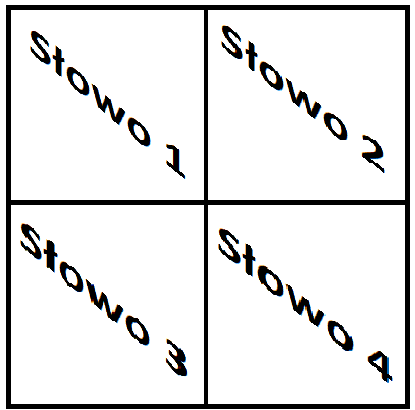
\includegraphics[width=8cm]{rys/gra5.png}
		\caption{Kod - Tryb graficzny}
		\label{rys:rysunek001}
	\end{center}
\end{figure}

	\begin{figure}[!htb]
	\begin{center}
		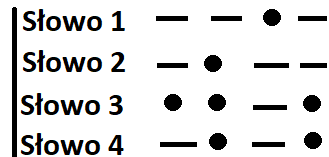
\includegraphics[width=8cm]{rys/gra6.png}
		\caption{Kod - Tryb tekstowy}
		\label{rys:rysunek001}
	\end{center}
\end{figure}
\hspace{-0.60cm}Trzeci tryb gry, który zostanie zaimplementowany do gry będzie oparty na latarce zawartej w telefonie. Telefon osoby obsługującej tryb graficzny włączy i wyłączy latarkę określoną liczbę razy tworząc przy tym "kod morsa" opisany w trybie tekstowym. Gracz obsługujący tryb graficzny będzie miał za zadanie zapamiętać stosunkowo krótki kod i podać go osobie będącej w trybie graficznym. Następnie osoba zarządzająca trybem graficznym musi dopasować go do jednego ze słów po czym podaje słowo kluczowe wspólnikowi. Wybór złego słowa pozbawia nas jednego życia i losuje nowy sygnał.
\\
\\
Kolejnym trybem gry będą "Kolorki". Będzie on polegał na odtworzeniu określonej sekwencji po jej wyświetleniu. Utrudnieniem będzie to, że każdy kolor będzie odpowiadał innemu, co będzie opisane w trybie graficznym. Gracz trybu graficznego będzie miał za zadanie komunikowania partnerowi jaki kolor został wyróżniony po czym kliknięcie w jego odpowiednik opisany w trybie tekstowym.
\\
\\
Ostatnia zagadka będzie stosunkowo prosta, będzie ona polegała na przytrzymaniu przycisku przez określony czas wtedy kiedy timer jako ostatnią cyfrę będzie miał cyfrę przypisaną do określonego koloru przycisku. Wszysko co musi wtkonać gracz w trybie graficznym jest opisane w trybie tekstowym.

\subsubsection{Tryb Graficzny}
Będzie opierał się na rozwiązywaniu zagadek. Gracz sam nie będzie w stanie rozwiązać zagadki, ponieważ podpowiedzi czy też cała solucja danej zagadki będą zawarte w trybie tekstowym.
W tym trybie będziemy widzieć plansze rozgrywki i będziemy mogli sterować naszą postacią.
\\
	\begin{figure}[!htb]
	\begin{center}
		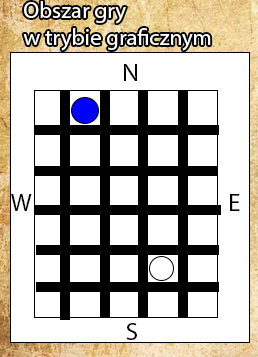
\includegraphics[width=8cm]{rys/gra2.png}
		\caption{Labirynt}
		\label{rys:rysunek001}
	\end{center}
\end{figure}

\hspace{-0.60cm}W trybie graficznym, jak widać na powyższym rysunku, widzimy naszą postać, niebieską kulkę, i nasz cel, białą kulkę. Natomiast nie widzimy drogi do mety~i w tym celu musimy komunikować się z partnerem.
\\
\\
Za każdym razem jak wykonamy zły ruch czyli wejdziemy w ścianę nasza kulka będzie wracać na początek trasy a my tracimy jedno z naszych żyć. Po utracie wszystkich żyć kończymy rozgrywkę.
\\
\\
Innym trybem gry będą literaki polegające na układaniu słów. Gracz w tym trybie będzie za pomocą strzałek zmieniał litery na określonych pozycjach. Błędna kombinacja prowadzi do utraty życia i jest równoznaczna z wejściem w ścianę w trybie labiryntu.
\\
\\
Tryb graficzny trzeciej gry będzie oparty na prostej tabeli z paroma różnymi opcjami do wyboru. W zależności od otrzymanych instrukcji od naszego wspólnika będziemy musieli wybrać jedną z nich. Telefon gracza obsługującego ten tryb będzie za pomocą latarki wyświetlał jeden z dwóch rodzajów sygnału. Bedzie to kod oparty o~kod morsa ale ze zmienionymi słowami. Dla przykładu jeżeli latarka włączy się raz na długo a potem 3 razy mrugnie będzie to oznaczało jeden sygnał długi (oznaczenie w trybie tekstowym - kreska) i 3 krótkie (w trybie tekstowym - kropka).
\\
\\
W trybie graficzny w czwartej zagadce będziemy musieli obserwować, który kolor zostaje wyróżniony. Następnie komunikujemy się z partnerem, który wskazuje nam odpowiadający kolor dla wyróżnionego po czym go klikamy. Sekwencja wydłuża się do pięciu wyróżnionych kolorów. Gra kończy się wraz ze zgadnięciem pięciu odpowiednich kolorów.
\\
\\
Ostatnia zagadka będzie stosunkowo prosta. Wymagane będzie od nas tylko przytrzymanie przycisku przez odpowiednio długi czas.
\subsubsection{Tryb Tekstowy}  %1.2

Będzie opierał się na znajdowaniu podpowiedzi czy też solucji do aktualnie wykonywanej zagadki przez osobę obsługującą tryb graficzny.
Naszym zadaniem będzie współpraca z osobą, która steruje postacią w trybie graficznym w celu jak najefektywniejszego ukończenia zagadek przed końcem ustalonego czasu.
\\
\\
\\
\begin{figure}[!htb]
	\begin{center}
		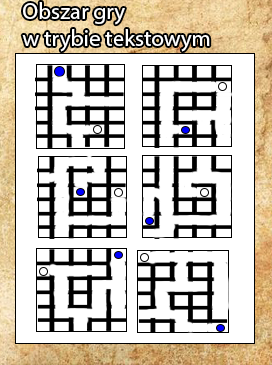
\includegraphics[width=8cm]{rys/gra3.png}
		\caption{Labirynt}
		\label{rys:rysunek001}
	\end{center}
\end{figure}

\hspace{-0.60cm}Jak można zobaczyć na rysunku 1.6 w trybie tekstowym będziemy widzieć dostępne mapy rozgrywki. Zadaniem gracza w trybie teksowym będzie takie poprowadzenie partnera w trybie graficznym, żeby niebieska kula dotarła do~mety (białej kuli) unikając wchodzenia w ściany. 
\\
\\
W trybie gry "Literaki"~gracz (obsługujący tryb tekstowy) będzie miał dostępną bazę ze słowami i będzie musiał dzięki komunikacji z graczem operującym interfejsem graficzym pomóc mu ułożyć pasujące słowo. Gracz w trybie graficznym będzie miał opcję ułożenia tylko jednego słowa z bazy.
 \\
 \\
 W trzecim trybie gry będziemy musieli za pomocą komunikacji z naszym partnerem rozszyfrować o jaki kod chodzi w danym momencie. W trybie tekstowym będziemy otrzymywać informacje dotyczące "wyglądu kodu". W rzeczywistości ostrzymamy informację ile było długich sygnałów a ile krótkich i w jakiej kolejności. Po otrzymaniu takowych informacji gracz będzie stawał przed wyborem jednego ze słów, które w tym przypadku będzie oznaczone przed chwilą otrzymanym kodem. Jeżeli żadne słowo się nie będzie zgadzać to najprawdopodobniej otrzymaliśmy złe podpowiedzi od naszego partnera. Jeżeli jednak znajdujemy pasujący kod to podajemy słowo, które ten kod opisuje do operatora trybu graficznego. 
 \\
 \\
 W czwartej zagadce będziemy mieli opisane, który kolor odpowiada któremu. Dla przykładu jeżeli zostanie wyróżniony kolor zielony to naszym zadaniem będzie poszukanie, który kolor jest przypisany do niego (na przykład czerwony) i zakomunikowanie tego naszemu partnerowi.
 \\
 \\
 W piątej zagadce będziemy mieli opis jaki kolor przycisku odpowiada ilości przytrzymanych sekund i jaka musi być ostatnia cyfra na timerze. Po sprawdzeniu tego przekazujemy naszemu partnerowi wszyskie te informacje a on kończy w ten sposób grę.
 
 
 
   \newpage
\section{Określenie wymagań szczegółowych}		%2
%Dokładne określenie wymagań aplikacji (cel, zakres, dane wejściowe) – np. opisać przyciski, czujniki, wygląd layautu, wyświetlenie okienek. Opisać zachowanie aplikacji – co po kliknięciu, zdarzenia automatyczne. Opisać możliwość dalszego rozwoju oprogramowania. Opisać zachowania aplikacji w niepożądanych sytuacjach.
\subsection{Założenia główne}
\begin{itemize}
\item \textbf{Utrzymanie modułowości projektu }
\item \textbf{Łatwość implementacji } 
\item   \textbf{Prostota w testowaniu i ewentualnym debuggingu}
\item \textbf{Podzielenie aplikacji na 2 tryby}
\item\textbf{ Użycie latarki}
\end{itemize}

\subsubsection{Utrzymanie modułowości projektu}
\hspace*{0.60cm}Pozwoli to na pracę nad wieloma "poziomami" jednocześnie co przełoży się na lepsze rozłożenie pracy pomiędzy członków grupy.

\subsubsection{Latwość implementacji}
\hspace*{0.60cm}Pozwoli to na testowanie każdego modułu osobno. Dzięki temu rozwiązaniu będziemy mogli lepiej wyeliminować błędy. A co za tym idzie lepiej dopracować nasz projekt.

\subsubsection{Prostota w testowaniu i ewentualnym debuggingu}
\hspace*{0.60cm}Chcemy dążyć do jak najłatwiejszego i jednocześnie najbardziej efektywnego sposobu testowania aplikacji. Pozwoli nam to zaoszczędzić cenny czas, który będziemy mogli poświęcić na lepsze dopracowanie szczegółów.

\subsubsection{Podzielenie aplikacji na 2 tryby}
\hspace*{0.60cm}Jednym z głównych rozwiązań w aplikacji będzie podzielenie jej na 2 zależne od siebie tryby (tryb graficzny i tekstory) zamiast tworzenia osobniej aplikacji dla każdego z trybów.
\\
\\
Jedną z wielu zalet tego rozwiązania będzie zmiejszenia nakładów pracy dzięki skupienu się tylko na jednej aplikacji. Dzięki temu aplikacja będzie bardziej dopracowana pod względem działania czy też wyglądu.
\\
\\
Drugą zaletą będzie łatwiejsze przeszukiwanie aplikacji pod względem błędów, testowanie jej czy też naprawa potencjalnych błędów, ponieważ nie trzeba będzie naprawiać tego samego błędu niekiedy w obydwu aplikacjach.
\\
\\
Trzecią zaletą będzie łatwość korzystania z aplikacji - obydwaj graczę muszą posiadać tą samą grę a nie dwie różne wersje. Dzięki temu łatwiej będzie można zamienić się trybem gry z partnerem co może zwiększyć radość z gry


\subsubsection{Użycie latarki}
Jedna z zagadek będzie oparta na wysyłaniu sygnałów w formnie kodu morsa za pomocą latarki. Latarka będzie uruchamiana na określony odstęp czasu po czym zostanie wyłączona i włączona ponownie jeżeli ostatni sygnał nie został pokazany. Kod będzie oparty na 2 sygnałach: krótkim i długim.

\subsection{Struktura aplikacji}

\hspace*{0.60cm}W aplikacji będzie dostępne:
\begin{itemize}
	\item \textbf{Menu główne}
	\item \textbf{Menu ustawień} 
	\item   \textbf{Dwa tryby gry}
\begin{itemize}
	\item \textbf{Tryb graficzny}
	\item \textbf{Tryb tekstowy} 
\end{itemize}
\end{itemize}

\subsubsection{Menu główne}
\hspace*{0.60cm}W tym panelu będziemy mieli dostęp zarówno do wyboru trybu gry jak i do ustawień
Ten panel będzie przejrzysty i łatwy w obsłudze, wszyskie opcje będą podpisane lub będą zawierały adekwatną do nazwy ikonę. Dla przykładu ustawienia zostaną oznaczone zębatką z podpisem ustawienia. Menu główne już na początku będzie zawierać jedną łatwą zagadkę

\subsubsection{Menu ustawień}
\hspace*{0.60cm}Ten panel umożliwi użytkownikom, jak sama nazwa wskazuje, ustawienia rozgrywki takie jak głośność muzyki. Do palenu ustawień będzie można wejść z każdego innego panelu. Zmiana ustawień będzie działała globalnie czyli zmiana głośności poskutuje zmianą głośności w każdym pozostałym panelu, do którego przejdziemy.

\subsubsection{Dwa tryby gry}
\hspace*{0.60cm}Użytkownicy będą mieli do wyboru tryb gry. Jeżeli użytkownik zdecyduje się na wybór trybu graficznego jedyne co będzie musiał zrobić to kliknąć w odpowieni przycisk oznaczony jako tryb graficzny. Tryby gry będą podpisane i każdy z nich będzie miał osoby panel odpowiadający za określone funkcję, które będą potrzebne do rozwiązania zagadki
   	\newpage
\section{Projektowanie}		%3
%Opis przygotowania narzędzi (git, visual studio). Wybór i opis bibliotek, klas. Szkic layoutów. Pseudo kody. Opisy wykorzystanych algorytmów (np. algorytm sortowania). Dokładniejsze określenie założeń i działania aplikacji, (np.: ten przycisk otworzy takie okno a w tym oknie wpisujemy takie dane).

\subsection{Wykorzystane narzędzia}

\hspace*{0.60cm}Podczas tworzenia aplikacji, której docelowym środowiskiem będzie Android wykorzystaliśmy platformę open source Xamarin i zestaw narzędzi Xamarin Community Toolkit, który ułatwił wykonywanie niektórych zadań. Projekt jest tworzony \\w języku C\# co umożliwia nam wykorzystanie Microsoft Visual Studio Community Edition 2022. IDE (z ang. Integrated Development Environment), czyli zintegrowane środowisko programistyczne posłuży nam do łatwiejszego modułowania aplikacji. Wszystkie wersje kodów aplikacji znajdują się na platformie GitHub dzięki czemu łatwiej będzie wrócić do poprzednich wersji aplikacji w przypadku wystąpienia błędów w działaniu aktualnej. Wszystko początkowo miało zostać połączone za pomocą bazdy danych Firebase. Baza ta umożliwiałaby przesyłanie danych między graczami i ułatwiała przejście do następnych poziomów.

\subsubsection{Xamarin}

\hspace*{0.60cm}Xamarin\footnote{ http://xamarinlab.pl/} (logo - rys. 3.1) to platforma typu open source do tworzenia nowoczesnych i wydajnych aplikacji dla systemów iOS, Android i Windows za pomocą platformy .NET. Xamarin to warstwa abstrakcji, która zarządza komunikacją udostępnionego kodu z bazowym kodem platformy. Środowisko Xamarin działa w środowisku zarządzanym, które zapewnia wygody, takie jak alokacja pamięci i odzyskiwanie pamięci.

	\begin{figure}[!htb]
	\begin{center}
		
\includegraphics[width=8cm]{rys/xamarin.png}
		\caption{Xamarin}
		\label{rys:rysunek001}
	\end{center}
\end{figure}

\subsubsection{Xamarin Community Toolkit}

\hspace*{0.60cm}Zestaw narzędzi Xamarin Community Toolkit\footnote{https://learn.microsoft.com/pl-pl/xamarin/community-toolkit/} (logo - rys 3.2)to zbiór elementów wielokrotnego użytku na potrzeby tworzenia aplikacji mobilnych za pomocą zestawu narzędzi Xamarin.Forms, w tym animacji, zachowań, konwerterów, efektów i pomocników. Upraszcza i demonstruje typowe zadania deweloperskie podczas kompilowania aplikacji dla systemów iOS, Android, macOS, WPF i platforma uniwersalna systemu Windows (UWP) przy użyciu platformy Xamarin.Forms.

	\begin{figure}[!htb]
	\begin{center}
		
\includegraphics[width=8cm]{rys/xtools.png}
		\caption{Xamarin Community ToolKit}
		\label{rys:rysunek001}
	\end{center}
\end{figure}

\subsubsection{Microsoft Visual Studio}

\hspace*{0.60cm}Microsoft Visual Studio\footnote{ https://visualstudio.microsoft.com/pl} (logo - rys 3.3) to zintegrowane środowisko programistyczne, służące do tworzenia, edytowania i debugowania kodu. IDE (z ang. Integrated Development Environment), czyli zintegrowane środowisko programistyczne to software oferujący szereg funkcji przydatnych podczas tworzenia oprogramowania dla systemów Windows, Android, iOS, rozwiązań internetowych oraz opartych \\o chmurę. Poza standardowym edytorem oraz debugerem, które zapewnia większość aplikacji IDE, program Microsoft Visual Studio zawiera jeszcze kompilatory, narzędzia do uzupełniania kodu i wiele innych funkcji usprawniających pracę.
\\
\\
\\
\\
\\
\\
\\
	\begin{figure}[!htb]
	\begin{center}
		
\includegraphics[width=8cm]{rys/visual.png}
		\caption{Visual}
		\label{rys:rysunek001}
	\end{center}
\end{figure}

\subsubsection{Git, GitHub}

\hspace*{0.60cm}Git jak i GitHub\footnote{ https://github.com/}  (logo - rys 3.4) to najczęściej używany nowoczesny system kontroli wersji. Za pomocą usługi Git możesz śledzić zmiany kodu wprowadzane \\w czasie i przywrócić określone wersje. Ponadto pozwala kontrolować dostęp do danych, wspiera zarządzanie wieloma repozytoriami. Jest to rozwiązanie, które pozwala zaoszczędzić sporo czasu i nerwów. Kolejnym plusem jest to, że jest on \\w miare łatwy w użyciu i jest przejrzysty. 
\\
\\
\\
\\
\\
\\
\\
\\
\\
	\begin{figure}[!htb]
	\begin{center}
		
\includegraphics[width=8cm]{rys/git.png}
		\caption{GitHub}
		\label{rys:rysunek001}
	\end{center}
\end{figure}


\subsubsection{Język C\#}

\hspace*{0.60cm}Język C\#\footnote{ https://learn.microsoft.com/pl-pl/dotnet/csharp/} (logo - rys 3.5) to zorientowany obiektowo język programowania, który umożliwia programostom tworzenie różnych bezpiecznych i niezawodnych aplikacji w środowisku .NET. Język ten udostępnia konstrukcje językowe, które bezpośrednio obsługują te koncepcje, dzięki czemu język C\# jest językiem naturalnym, w którym można tworzyć składniki oprogramowania i ich używać.
\\
\\
\\
\\
\\
\\
\\
\\
\\
\\
\\
\\
\\
\\
\\
\\
\\
\\
	\begin{figure}[!htb]
	\begin{center}
		
\includegraphics[width=8cm]{rys/c.png}
		\caption{C\#}
		\label{rys:rysunek001}
	\end{center}
\end{figure}
\subsubsection{Baza danych SQLite}
\hspace*{0.60cm}SQLite\footnote{ https://www.sqlite.org/index.html} (logo - rys 3.6) jest bez serwerową, relacyjną, lekką bazą danych. Znajduje się w dokładnie jednych pliku. Bardzo często wybierana jako baza dla aplikacji iOS oraz Android. 
Zawartość bazy danych przetrzymywana jest w jednym pliku. Baza SQLite jest utrzymywana na dysku przy użyciu B-drzew. Osobne drzewo jest używane dla każdej z tabel i każdego z indeksów. Baza udostępnia transakcje ACID oraz implementuje większość standardu SQL 92. Jest często wykorzystywany w większych aplikacjach oraz w systemach obsługi relacyjnych baz danych takich jak Kexi.
\\
	\begin{figure}[!htb]
	\begin{center}
		
\includegraphics[width=8cm]{rys/baza.png}
		\caption{Komunikat błędu}
		\label{rys:rysunek001}
	\end{center}
\end{figure}
\\
\subsection{Działanie aplikacji}
\hspace*{0.60cm}Gra zawiera kilka paneli:
\begin{itemize}
	\item \textbf{Menu główne}
	\item \textbf{Menu ustawień} 
	\item   \textbf{Dwa tryby gry}
	\begin{itemize}
		\item \textbf{Tryb graficzny}
		\item \textbf{Tryb tekstowy} 
	\end{itemize}
\end{itemize}


\subsubsection{Menu główne}
Po uruchomieniu aplikacji powita nas już pierwsza zagadka (rys 3.7), która polega na znalezienu przycisku pozwalającego przejść dalej. Tym przyciskiem jest przycisk oznaczony żarówką. Jeśli jednak zostanie wciśnięty duży czerwony przycisk na środku ekranu to gra zostanie wyłączona. 
\\Jak widać mamy dostępny jeszcze przycisk oznaczony zębatką. Prowadzi on do ustawień rozgrywki.
\\
\\
\\
\\
\\
\\
\\
\\
\\
\\
\\
\\
\\
\\
\\
\\
\\
\\
	\begin{figure}[!htb]
	\begin{center}
		
\includegraphics[width=8cm]{rys/menu1.png}
		\caption{Menu Główne}
		\label{rys:rysunek001}
	\end{center}
\end{figure}

	\begin{figure}[!htb]
	\begin{center}
		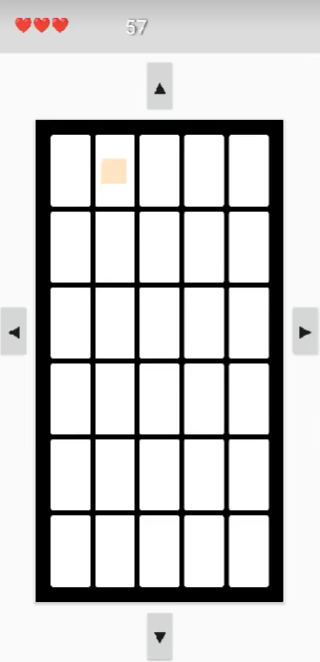
\includegraphics[width=8cm]{rys/menu12.png}
		\caption{Menu Główne v2}
		\label{rys:rysunek001}
	\end{center}
\end{figure}

Po wciśnięciu dobrego przycisku przechodzimy do właściwego menu głównego (rys 3.8), w którym możemy przejść dalej 
\\
\\
\\
\\
\\
\\
\\

\subsubsection{Ustawienia}
\hspace*{0.60cm}Ten panel (rys. 3.9) oferuje nam zmianę ustawień gry. Dla przykładu głośności muzyki. Po zmienieniu głośności w panelu ustawień wartość ustawiona zostaje zapisana i przenoszona na inne panele aplikacji. Przejście do menu ustawień będzie możliwe zarówno z menu głównego jak i z poziomu gry.
	
	\begin{figure}[!htb]
	\begin{center}
		
\includegraphics[width=8cm]{rys/ustawienia.png}
		\caption{Ustawienia}
		\label{rys:rysunek001}
	\end{center}
\end{figure}


\subsubsection{Tryb graficzny}
\hspace*{0.60cm}Pierwsza zagadka w trybie graficznym będzie wyglądała tak jak na rys 3.10.
Pomarańczowy kwdrat jest naszą postacią, którą poruszamy za pomocą strzałek umieszczonych na ekranie.
Każda strzałka odpowiada za ruch w inną stronę.
\\
\\
\\
\\
	\begin{figure}[!htb]
	\begin{center}
		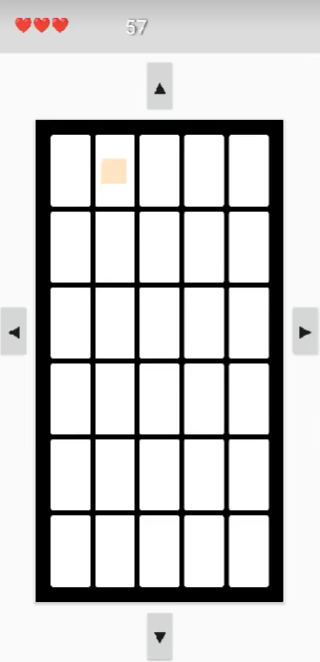
\includegraphics[width=8cm]{rys/gra7.png}
		\caption{Labirynt}
		\label{rys:rysunek001}
	\end{center}
\end{figure}

\hspace*{0.60cm}Kolejna zagadka będzie polegała na wyborze odpowiedniego słowa, będziemy zamieniać litery za pomocą strzałek jak na rys 3.11. Jeżeli ułożymy odpowiednie słowo zatwierdzamy przyciskem oznaczonym "ptaszkiem". Za pomocą przycisku odtwórz możemy odtworzyć kod morsa z latarki od nowa.

	\begin{figure}[!htb]
	\begin{center}
		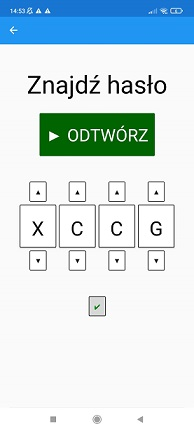
\includegraphics[width=8cm]{rys/gra8.png}
		\caption{Literaki}
		\label{rys:rysunek001}
	\end{center}
\end{figure}

   	\newpage
\section{Implementacja}		%4

\subsection{Przycisk}
Przyciski to podstawowy i najprostszy element większości aplikacji. Ten element poprzez klikanie w niego wykonuje określoną akcje. Kod przykładowego przycisku w naszej grze można znaleźć na listungu 1:

\begin{lstlisting}[caption=Button]
	<Button Grid.Row="0" 
	Grid.Column="0" 
	Text="&#x2699;" 
	x:Name="SettingsButton" 
	Padding="0,0,2,2" 
	FontAttributes="Bold"  
	FontSize="24" 
	Clicked="GoToSettings"></Button>
\end{lstlisting}

\subsubsection{Użyte atrybuty przycisku (listing 1)}
\begin{itemize}	
	\item \textbf{Grid }- ustawia element na "siatce",
	\begin{itemize}
	\item \textbf{Grid.Row (linia 1)  }- odpowiada za oś Y czyli rząd,
	\item \textbf{Grid.Column (linia 2) }- odpowiada za oś X czyli kolumnę,
	\end{itemize}
	\item \textbf{Text (linia 3) }- napis wewnątrz przycisku. W tym wypadku kod szesnastkowy (hexcode) zębatki,
	\item \textbf{Padding (linia 5) }- wewnętrzny margines,
	\item \textbf{FontSize (linia 7) }- rozmiar czcionki,
	\item \textbf{Clicked (linia 8)} - przycisk po kliknięciu odwołuje się do metody o tej nazwie,
	\item \textbf{CornerRadius} - zaokrągla rogi przycisku, przy odpowiednio dużej wartości, przicisk może stać się okrągły.

	
\end{itemize}
\subsubsection{Inne użyteczne atrybuty}
\textbf{Można znaleźć na listingu 2. Opisują one polecenie label.}
\begin{itemize}
	\item \textbf{X:Name (linia 3) }- nazwa elementu używana potem w C\#,
	\item \textbf{Vertical/HorizontalTextAlignment (linia 6)} - ustawia test na osi X/Y w zależności od wybranej opcji,
	\item \textbf{BackgroundColor (linia 8)} -pozwala na zmianę koloru tła.
\end{itemize}

\begin{lstlisting}[caption=Label]
	<Label Grid.Row="0" 
	Grid.Column="0" 
	x:Name="Tit" 
	Text="TytuL" 
	Grid.ColumnSpan="4" 
	VerticalTextAlignment="Center" 
	HorizontalTextAlignment="Center" 
	BackgroundColor="White"/>
	
\end{lstlisting}
\subsubsection{Przyciski w formie zdjęcia}
Inna forma wstawiania przyciusku, w którym zamiast tekstu znajdziemy wstawione zdjęcie jest pokazana na listingu 3.
\begin{lstlisting}[caption=ImageButton]
<ImageButton Grid.Column="0" Grid.Row="0" x:Name="BulbButton" Clicked="ChangeLight" ClassId="0" 
Source="https://cdn-icons-png.flaticon.com/512/74/74072.png" Aspect="AspectFit" IsVisible="true" >
	<VisualStateManager.VisualStateGroups>
		<VisualStateGroup x:Name="CommonStates">
			<VisualState x:Name="Normal">
				<VisualState.Setters>
					<Setter Property="Scale" Value="1" />
				</VisualState.Setters>
			</VisualState>
			<VisualState x:Name="Pressed">
				<VisualState.Setters>
					<Setter Property="Scale" Value="0.8" />
				</VisualState.Setters>
			</VisualState>
		</VisualStateGroup>
	</VisualStateManager.VisualStateGroups>
</ImageButton>
\end{lstlisting}

\subsubsection{Użyte atrybuty}
\begin{itemize}
	\item \textbf{VisualState  (linie 3-16)} - pozwala na zmianę wyglądu w zależności od stanu przycisku. W naszym przypadku state "normal" odnosi się do domyślnego ustawienia. State "Pressed" sprawia, że skala obiektu zmienia się do 0.8 (zmniejsza się, linia 12) symulując efekt naciśnięcia po czym wraca do state "normal",
	\item \textbf{Source (linia 2)} - źródło obrazka, w tym wypadku link ale możliwe jest też użycie ścieżki. 
\end{itemize}
\subsection{MainPage}
Funkcja pokazana na listingu 4 służy do sprawdzenia czy jest ustalona wartość głośności muzyki, a następnie ustawia w linii 6 wartość Volume soundtracku właśnie jako tą wartość.

\begin{lstlisting}[caption=MainPage]
public MainPage(double dalej)
{
	InitializeComponent();
	if (dalej == 0)
	dalej = 1;
	soundtrack.Volume = dalej;
}
\end{lstlisting}

\subsection{OnAppearing}
Na listingu 5 nadpisujemy metodę OnAppearing(), która wykonuje się na starcie.
\\
Metoda FindByName znajduje elementy o podanych nazwach, na następnie wykonuje dla nich metodę Animate\_Pulse().
\\
Do zmiennej status przypisany zostaje stan "Uprawnienia do używania aparatu"~przez aplikację (potrzebne do użycia lampy błyskowej).
\\
Następnie w linii 16 sprawdzany jest status. Jeżeli status jest nieznany (unknown) lub odmówiono dostępu aplikacja prosi o przyznanie takiego uprawnienia.

\begin{lstlisting}[caption=OnAppearing]
async protected override void OnAppearing()
{
	base.OnAppearing();
	arrow_1 = (Label)FindByName("arrow_1");
	arrow_2 = (Label)FindByName("arrow_2");
	arrow_3 = (Label)FindByName("arrow_3");
	arrow_4 = (Label)FindByName("arrow_4");
	bigRed = (Button)FindByName("bigRed");
	BulbButton = (ImageButton)FindByName("BulbButton");
	Animate_pulse(arrow_1);
	Animate_pulse(arrow_2);
	Animate_pulse(arrow_3);
	Animate_pulse(arrow_4);
	animate_button(bigRed);
	var status= await Permissions.CheckStatusAsync<Permissions.Camera>();
	if (status==PermissionStatus.Unknown || status == PermissionStatus.Denied)
	{
		await Permissions.RequestAsync<Permissions.Camera>();
	}
}
\end{lstlisting}

\subsection{Animate\_pulse}
Animate\_pulse zawarte na listingu 6 włącza animacje, w której to skala strzałek zmienia się pomiędzy 1 a 1.2.
\\
W tym przypadku używane jest ClassId po to, by nazywać animacje różnymi nazwami (te same nazwy nadpisywałby się).
\\
W tym przypadku, przez połowę czasu animacji skala rośnie, by przez drugą połowę maleć.

\begin{itemize}
	\item \textbf{  This (linia 9) } – Animacja, która będzie animowana,   
	\item \textbf{  Objname (linia 10) } – nazwa służąca jako uchwyt do animacji,  
	\item \textbf{  16 (linia 11) } – Czas w milisekundach pomiędzy elementami animacji,  
	\item \textbf{  950 (linia 12) } – czas w milisekundach trwania animacji,   
	\item \textbf{  Easing.Linear (linia 13) } – funkcja używana do opisu animacji, 
	\item \textbf{  (v,c) =>>obj.Scale=1 (linia 14) } – co ma zostać wykonane po skończeniu animacji ,  
	\item \textbf{  ()=>>true (linia 15) } – czy funkcja ma być zapętlona.   
\end{itemize}

\begin{lstlisting}[caption=Animate\_pulse]
void Animate_pulse(Label obj)
{
	var Objname = obj.ClassId;
	var a = new Animation {
		{0,0.5, new Animation(v => obj.Scale = v, 1, 1.2) },
		{0.5,1, new Animation(v => obj.Scale = v, 1.2, 1) }
	};
	a.Commit(
	this,
	Objname,
	16,
	950,
	Easing.Linear, 
	(v, c) => obj.Scale = 1,
	()=> true);
}
\end{lstlisting}

\subsection{FirstTask}
Funkcja zawarta na listingu 7 to funkcja, przyjmująca jako parametry obiekt, który został wciśnięty i argumenty zdarzenia, pozwala na przemieszczanie się pomiędzy stronami aplikacji.
\\
Metoda soundtrack.Stop() (linia 3) sprawia, że soundtrack przestaje grać.
\\
Do zmiennej dalej (linia 4) przekazywana jest aktualna wartość głośności muzyki granej w tle.
\\
Następnie (linia 5) asynchronicznie przechodzimy do nowej strony, przekazując jako parametr głośność soundtracku, by ten mógł grać z taką samą głośnością jaka była ustawiona.

\begin{lstlisting}[caption=FirstTask]
private async void FirstTask(object sender, EventArgs e)
{
	soundtrack.Stop();
	double dalej1 = soundtrack.Volume;
	await Navigation.PushAsync(new LabirynthPage(dalej1));
}
\end{lstlisting}

\subsection{Wciśnięcie złego przycisku}
Funkcja na listingu 8 odpowiada za wciśnięciu złego przycisku. Po wciśnięciu go zmienia się widoczność wszystkich elementów menu, następnie wyświetla się obrazek świadczący o porażce (linia 17), a po odczekaniu 3,5s (linia 19) proces aplikacji kończy się i zwraca wartość 0, co świadczy o poprawnym zamknięciu aplikacji (linia 20).

\begin{lstlisting}[caption=WrongButton]
async void WrongButtonClicked(object sender, EventArgs e)
{
	ChangeLight(sender,e);
	var ButtonDalej = (Button)FindByName("LabirynthButton");
	var bulbButton = (ImageButton)FindByName("BulbButton");
	var settingsButton= (Button)FindByName("SettingsButton");
	var deadAnimation = (Image)FindByName("deadAnimation");
	var ButtonLatarka = (Button)FindByName("FlashlightButton");
	var ButtonTekstowy = (Button)FindByName("TextModeButton");
	var ButtonMorse = (Button)FindByName("ButtonMorse");
	ButtonDalej.IsVisible = false;
	ButtonTekstowy.IsVisible = false;
	ButtonLatarka.IsVisible = false;
	ButtonMorse.IsVisible = false;
	bulbButton.IsVisible = false;
	settingsButton.IsVisible = false;
	deadAnimation.IsVisible = true;
	deadAnimation.IsAnimationPlaying = true;
	await Task.Delay(3500);
	System.Environment.Exit(0);
}
\end{lstlisting}

\subsection{HUD}
HUD (ang. heads-up display) – Ważna część gier komputerowych. Jest to sekcja zawierająca informacje na temat rozgrywki, pozwalająca graczowi na odnalezienie informacji o niej. Nazwa wywodzi się od tzw. wyświetlacza przeziernego HUD stosowanego np. przez pilotów samolotów bojowych.
\\
W linach 5-7 są opisane życia w postaci serc.
\\
Linie 8-9 są odpowiedzialne za timer, jego widoczność, przezroczystość i cień jaki rzuca.
\begin{lstlisting}[caption=HUD]
            <Frame Grid.Row="0" Grid.ColumnSpan="20" Grid.RowSpan="2" BackgroundColor="Gray">
<Grid>
<Label Grid.Column="0"></Label>

<Label Grid.Column="0" TextColor="White"  FontSize="30" VerticalTextAlignment="Center" x:Name="HealthBar1" Text="&#10084;"></Label>
<Label Grid.Column="1" TextColor="White"  FontSize="30" VerticalTextAlignment="Center" x:Name="HealthBar2" Text="&#10084;"></Label>
<Label Grid.Column="2" TextColor="White"  FontSize="30" VerticalTextAlignment="Center" x:Name="HealthBar3" Text="&#10084;"></Label>

<Label x:Name="Timer" Margin="0,0,0,15"  Grid.Column="3" Grid.ColumnSpan="3"  TextColor="White" VerticalTextAlignment="Center" xct:ShadowEffect.Color="Black" xct:ShadowEffect.Opacity="0.7" xct:ShadowEffect.OffsetX="5" xct:ShadowEffect.Radius="5" FontSize="25" FontAttributes="Bold"></Label>
<Label x:Name="TimerCount" xct:ShadowEffect.Color="Black" xct:ShadowEffect.Opacity="0.7" xct:ShadowEffect.OffsetX="5" xct:ShadowEffect.Radius="5" Margin="0" TextColor="White" Grid.Column="5" VerticalOptions="Center" FontSize="25"></Label>
<Label Grid.Column="5" Grid.ColumnSpan="3"  TextColor="White" VerticalTextAlignment="Center" x:Name="CodeNumber"></Label>

<Label Grid.Column="1"></Label>
</Grid>
</Frame>
\end{lstlisting}

\subsection{Literaki}
Linia 1 - zmienna zawierająca ilość "żyć" (podejść),
\\Linia 2 - tablica przechowująca indeks każdego z bloków,
\\Linia 3 - tablica przechowująca słowa mogące wystąpić jako rozwiązanie,
\\Linia 4 - tablica przechowująca wszystkie wartości indeksów każdego z bloków,
\\Linia 11 - zmienna zawierająca indeks wartości z TextTable[], która została wybrana jako rozwiązanie,
\\Linia 12 - zmienna zawierająca pozostały czas na rozwiązanie zagadki,
\\Linia 13 - zmienna zawierająca obiekt klasy Random, służący m.in. do losowania liczby z przedziału.
\begin{lstlisting}[caption=Literaki]
public int HealthCount = 3;
int[] BlockCounters = { 0, 0, 0, 0 };
readonly string[] TextTable = { "ARAB", "ALGA", "ALFA", "BAZA", "BETA", "BUDA", "BUNT", "GLON", "GONG", "GRAM", "LAWA", "LIRA", "LUFA", "RATA", "ROPA", "RYSY" };
public char[,] WordTable =
{
	{'A','A','A','A'},
	{'A','A','A','A'},
	{'A','A','A','A'},
	{'A','A','A','A'},
};
public int ChosenWord;
public int TimeLeft = 60;
Random RandomCharCount = new Random();
\end{lstlisting}

\subsection{SetTime}
W Linii 4 wyświetla się okno, które należy zamknąć, zanim ruszy zegar. Później uruchamiana jest metoda StartTimer(TimeSpan). TimeSpan przyjmuje trzy wartości - godziny, minuty i sekundy.
\\W Liniach 8-9 Odejmowane jest 1 od pozostałego czasu, a następnie uzyskana wartość jest wpisywana jako text do obiektu TimeCount.
\\W linii 10 widoczny jest warunek, który zmienia kolor tekstu na czerwony jeśli mamy mniej czasu niż 15 sekund, a w wypadku gdy się skończy czas wyświetla odpowiedni komunikat.
\begin{lstlisting}[caption=SetTime]
async void SetTime()
{
	await DisplayAlert("Rozpocznij zagadke", "Wcisnij OK, aby rozpoczac", "OK");
	Label TimeCount = (Label)FindByName("TimerCount");
	Label TimeBar = (Label)FindByName("Timer");
	Device.StartTimer(new TimeSpan(0, 0, 1), () =>
	{
		TimeLeft--;
		TimeCount.Text = TimeLeft.ToString();
		if (TimeLeft < 15)
		{
			TimeCount.TextColor = Color.Red;
			if (TimeLeft == 0)
			{
				DisplayAlert("Przegrales", "):", "No nie");
				TimeCount.Text = "";
				TimeBar.Text = TimeCount.Text;
				return false;
			}
		}
		return true;
	});
}

\end{lstlisting}

\subsection{SetColumns}
W każdej iteracji pętli do zmiennej name wpisywana jest nazwa Bloku, po czym w zmiennej Obj umieszczany jest obiekt o tej nazwie.
\\W Linii 6 Losowany jest liczba stałoprzecinkowa z zakresu 0 do rozmiaru tablicy WordTable.
\\W linii 7 jako wartość atrybutu text umieszczamy wylosowany znak.
\\Ta funkcja służy początkowemu ustawieniu tekstu w blokach.
\begin{lstlisting}[caption=SetColums]
setColumns()
{
	for (int i = 0; i < 4; i++)
	{
		var Name = "Block" + i;
		var Obj = (Label)FindByName(Name);
		var Los = RandomCharCount.Next(0, (WordTable.Length / 4) - 1);
		Obj.Text = WordTable[Los, i].ToString();
	}
}
\end{lstlisting}

\subsection{RandomizeWordTable}
W Linii 7 do zmiennej nextChar wpisywana jest losowa liczba z zakresu (65,90), która następnie zostaje przekonwertowana na char (są to znaki z zakresu [A-Z]) i~wpisana jako wartość tablicy WordTable - w ten sposób za każdym razem losowana jest cała tablica ze znakami.
\begin{lstlisting}[caption=RandomizeWordTable]
RandomizeWordTable()
{
	for (int i = 0; i < (WordTable.Length/4); i++)
	{
		for (int j = 0; j < 4; j++)
		{
			var nextChar = RandomCharCount.Next(65, 90);
			WordTable[i, j] = Convert.ToChar(nextChar);
		}
	}
	char[] chosenWordChars = TextTable[ChosenWord].ToCharArray();
	for (int i = 0; i < 4; i++)
	{
		int random = RandomCharCount.Next(1, (TextTable.Length/4) - 1);
		WordTable[random, i] = Convert.ToChar(chosenWordChars[i]);
	}
}	
\end{lstlisting}

\subsection{RandomizeText}
Sprawia, że do zmiennej ChosenWord wpisywana jest losowa liczba z zakresu od zera do długości tablicy ze słowami. Dzięki temu wylosowane zostało jedno słowo, które zostanie potem użyte jako hasło.
RandomizeWordTable().
\begin{lstlisting}[caption=RandomizeText]
	RandomizeWordTable()
	{
		for (int i = 0; i < (WordTable.Length/4); i++)
		{
			for (int j = 0; j < 4; j++)
			{
				var nextChar = RandomCharCount.Next(65, 90);
				WordTable[i, j] = Convert.ToChar(nextChar);
			}
		}
		char[] chosenWordChars = TextTable[ChosenWord].ToCharArray();
		for (int i = 0; i < 4; i++)
		{
			int random = RandomCharCount.Next(1, (TextTable.Length/4) - 1);
			WordTable[random, i] = Convert.ToChar(chosenWordChars[i]);
		}
	}	
\end{lstlisting}

\subsection{MoveUp}
Ta funkcja zbiera informacje na temat bloku o danym ClassId (każdy blok ma swój classId 0-3, classId jest takie same dla przycisku i bloku) i wysyła je do funkcji ChangeBlockText() z parametrem up. 
\begin{lstlisting}[caption=MoveUp]
	void MoveUp(object sender, EventArgs e)
	{
		var Button = (Button)sender;
		var Name = "Block" + Button.ClassId.ToString();
		var whichBlock = (Label)FindByName(Name);
		int ClassId = Convert.ToInt32(Button.ClassId);
		ChangeBlockText(whichBlock, ClassId, "up");
	}
\end{lstlisting}

\subsection{ChangeBlockText}
W zależności od podanego parametru, wartość indeksu BlockCounters[blockNumber] zwiększa się (dla parametru down) lub zmniejsza się (dla parametru up) sprawiając efekt "przewijania się"~po liście znaków. 
\\Jeżeli będziemy chcieli wyjść poza zakres znaków w tablicy, to wartość indeksu zmieni się na pierwszy (dla parametru dow) lub ostatni (dla parametru up).
\begin{lstlisting}[caption=ChangeBlockText]
	        void ChangeBlockText(Label block, int blockNumber, string where)
	{
		if (where == "up")
		{
			if (BlockCounters[blockNumber] == 0)
			{
				BlockCounters[blockNumber] = (WordTable.Length / 4) - 1;
			}
			else BlockCounters[blockNumber]--;
			
		}
		else if (where == "down")
		{
			if (BlockCounters[blockNumber] == (WordTable.Length / 4) - 1)
			{
				BlockCounters[blockNumber] = 0;
			}
			else BlockCounters[blockNumber]++;
		}
		block.Text = WordTable[BlockCounters[blockNumber], blockNumber].ToString();
	}
\end{lstlisting}

\subsection{CheckIfWin}
Ta funkcja sprawdza warunek zwycięstwa (ciąg znaków zgadza się z elementem z tablicy WordTable). 
\\W linii 4 ustawiana jest flaga WinFlag jako false (false oznacza brak zgodności, true zgodność). 
\\W liniach 5-10 odczytywana jest wartość z elementów Block0 - Block3, po czym jest to sklejane w jeden ciąg, umieszczony w zmiennej userGuess.
\\W liniach 11-17 iterujemy po wszystkich elementach tablicy WordTable (tam są słowa możliwe do uzyskania). 
\\W linii 13 umieszczony jest warunek, który sprawdza, czy wybrany przez użytkownika ciąg znaków jest zgodny z elementem z tablicy. Jeśli tak to flaga WinFlag przestawiana jest na "true".
\\W linii 18 sprawdzamy czy flaga ma wartość True. Jeśli tak, oznacza to wygraną. W przeciwnym razie zmniejszana jest liczba serc o 1.

\begin{lstlisting}[caption=CheckIfWin]
	 async void CheckIfWin(object sender, EventArgs e)
	{
		var userGuess = "";
		var WinFlag = false;
		for (int i = 0; i < 4; i++)
		{
			var Name = "Block" + i;
			var Block = (Label)FindByName(Name);
			userGuess += Block.Text;
		}
		for (int i = 0; i < TextTable.Length; i++)
		{
			if (TextTable[i] == userGuess)
			{
				WinFlag = true;
			}
		}
		if (WinFlag)
		{
			DisplayAlert("Kod do nastepnej zagadki to: ", "2115", "Ok");
			await Navigation.PushAsync(new FlashlightPage());
		}
		else
		{
			setHeartStatus();
			LoverHeartCount();
		}
	}
\end{lstlisting}

\subsection{MoveDown}
Ta funkcja zbiera informacje na temat bloku o danym ClassId (każdy blok ma swój classId 0-3, classId jest takie same dla przycisku i bloku) i wysyła je do funkcji ChangeBlockText() z parametrem down.
\begin{lstlisting}[caption=MoveDown]
        void MoveDown(object sender, EventArgs e)
{
	var Button = (Button)sender;
	var Name = "Block" + Button.ClassId.ToString();
	var whichBlock = (Label)FindByName(Name);
	int ClassId = Convert.ToInt32(Button.ClassId);
	ChangeBlockText(whichBlock, ClassId, "down");
}
\end{lstlisting}
   	\newpage
\section{Testowanie}	%5
%Opisujemy testy, sprawdzamy czy nie generuje błędów.
\textbf{Testy zostały wykonane według tabeli 5.1 i zostały w niej opisane}
\begin{longtable}{|c|c|c|}
	\caption{}
	\label{tab:my-table}\\
	\hline
	\multicolumn{1}{|c|}{Obiekt}                                                                                       & \multicolumn{1}{c|}{Opis działania}                                                                                                       & Poprawność działania \\ \hline
	\endfirsthead
	%
	\endhead
	%
	\multicolumn{1}{|c|}{\begin{tabular}[c]{@{}c@{}}Duzy czerwony przycisk \\ ("wciśnij mnie")\end{tabular}}           & \multicolumn{1}{c|}{Wyłącza aplikacje}                                                                                                    & Działa poprawnie     \\ \hline
	\multicolumn{1}{|c|}{Przycisk ustawień}                                                                            & \multicolumn{1}{c|}{Włącza menu ustawień}                                                                                                 & Działa poprawnie     \\ \hline
	\multicolumn{1}{|c|}{\begin{tabular}[c]{@{}c@{}}Przycisk przejścia dalej \\ (żarówka)\end{tabular}}                & \multicolumn{1}{c|}{Włacza prawdziwe menu główne}                                                                                         & Działa poprawnie     \\ \hline
	\multicolumn{1}{|c|}{Przycisk "Przejdź dalej"}                                                                     & \multicolumn{1}{c|}{Przechodzi dalej}                                                                                                     & Działa poprawnie     \\ \hline
	\multicolumn{1}{|c|}{\begin{tabular}[c]{@{}c@{}}Pasek zmiany głośności \\ (Menu ustawień)\end{tabular}}            & \multicolumn{1}{c|}{\begin{tabular}[c]{@{}c@{}}Podczas przesuwania  \\ zmienia wartość\end{tabular}}                                      & Działa poprawnie     \\ \hline
	\multicolumn{1}{|c|}{\begin{tabular}[c]{@{}c@{}}Przycisk zatwierdź \\ (Menu ustawień)\end{tabular}}                & \multicolumn{1}{c|}{\begin{tabular}[c]{@{}c@{}}Zapisuje wartość ustawioną \\  na pasku i przypisuje \\ ją dla każdej z kart\end{tabular}} & Działa poprawnie     \\ \hline
	\multicolumn{3}{|c|}{Labirynt}                                                                                                                                                                                                                                                        \\ \hline
	\multicolumn{1}{|c|}{\begin{tabular}[c]{@{}c@{}}Strzałka w lewo\\  (Labirynt)\end{tabular}}                        & \multicolumn{1}{c|}{Postać przemieszcza się w lewo}                                                                                       & Działa poprawnie     \\ \hline
	\multicolumn{1}{|c|}{\begin{tabular}[c]{@{}c@{}}Strzałka w prawo \\ (Labirynt)\end{tabular}}                       & \multicolumn{1}{c|}{Postać przemieszcza się w prawo}                                                                                      & Działa poprawnie     \\ \hline
	\multicolumn{1}{|c|}{\begin{tabular}[c]{@{}c@{}}Strzałka w górę \\ (Labirynt)\end{tabular}}                        & \multicolumn{1}{c|}{Postać przemieszcza się w górę}                                                                                       & Działa poprawnie     \\ \hline
	\multicolumn{1}{|c|}{\begin{tabular}[c]{@{}c@{}}Strzałka w dół \\ (Labirynt)\end{tabular}}                         & \multicolumn{1}{c|}{Postać przemieszcza się w dół}                                                                                        & Działa poprawnie     \\ \hline
	\multicolumn{1}{|c|}{\begin{tabular}[c]{@{}c@{}}Przejście labiryntu \\ (Wejście na odpowiednie pole)\end{tabular}} & \multicolumn{1}{c|}{Przenosi do innej zagadki}                                                                                            & Działa poprawnie     \\ \hline
	\multicolumn{1}{|c|}{Wejście w ścianę}                                                                             & \multicolumn{1}{c|}{\begin{tabular}[c]{@{}c@{}}Resetuje pozycję postaci \\ i odbiera jedno z żyć\end{tabular}}                            & Działa poprawnie     \\ \hline
	\multicolumn{3}{|c|}{Kod morsa}                                                                                                                                                                                                                                                        \\ \hline
	\multicolumn{1}{|c|}{\begin{tabular}[c]{@{}c@{}}Strzałka w górę\\ (Pierwsza)\end{tabular}}                         & \multicolumn{1}{c|}{\begin{tabular}[c]{@{}c@{}}Zmienia literę na \\ odpowiednim polu\end{tabular}}                                        & Działa poprawnie     \\ \hline
	\multicolumn{1}{|c|}{\begin{tabular}[c]{@{}c@{}}Strzałka w górę \\ (Druga)\end{tabular}}                           & \multicolumn{1}{c|}{\begin{tabular}[c]{@{}c@{}}Zmienia literę na \\ odpowiednim polu\end{tabular}}                                        & Działa poprawnie     \\ \hline
	\multicolumn{1}{|c|}{\begin{tabular}[c]{@{}c@{}}Strzałka w górę \\ (Trzecia)\end{tabular}}                         & \multicolumn{1}{c|}{\begin{tabular}[c]{@{}c@{}}Zmienia literę na\\ odpowiednim polu\end{tabular}}                                         & Działa poprawnie     \\ \hline
	\multicolumn{1}{|c|}{\begin{tabular}[c]{@{}c@{}}Strzałka w górę\\  (Czwarta)\end{tabular}}  & \multicolumn{1}{c|}{\begin{tabular}[c]{@{}c@{}}Zmienia literę na \\ odpowiednim polu\end{tabular}}                                                                                   & Działa poprawnie \\ \hline
	\multicolumn{1}{|c|}{\begin{tabular}[c]{@{}c@{}}Strzałka w dół\\ (Pierwsza)\end{tabular}}   & \multicolumn{1}{c|}{\begin{tabular}[c]{@{}c@{}}Zmienia literę na \\ odpowiednim polu\end{tabular}}                                                                                   & Działa poprawnie \\ \hline
	\multicolumn{1}{|c|}{\begin{tabular}[c]{@{}c@{}}Strzałka w dół\\ (Druga)\end{tabular}}      & \multicolumn{1}{c|}{\begin{tabular}[c]{@{}c@{}}Zmienia literę na \\ odpowiednim polu\end{tabular}}                                                                                   & Działa poprawnie \\ \hline
	\multicolumn{1}{|c|}{\begin{tabular}[c]{@{}c@{}}Strzałka w dół \\ (Trzecia)\end{tabular}}   & \multicolumn{1}{c|}{\begin{tabular}[c]{@{}c@{}}Zmienia literę na\\  odpowiednim polu\end{tabular}}                                                                                   & Działa poprawnie \\ \hline
  	\multicolumn{1}{|c|}{\begin{tabular}[c]{@{}c@{}}Strzałka w dół \\ (Czwarta)\end{tabular}}   & \multicolumn{1}{c|}{\begin{tabular}[c]{@{}c@{}}Zmienia literę na\\  odpowiednim polu\end{tabular}}                                                                                   & Działa poprawnie \\ \hline
	\multicolumn{1}{|c|}{Przycisk odtwórz}                                                      & \begin{tabular}[c]{@{}c@{}}Odtwarza kod morsa\\ za pomocą latarki\end{tabular}                                                                                                                           & Działa poprawnie \\ \hline
	\multicolumn{1}{|c|}{Zatwierdzenie hasła}                                                   & \multicolumn{1}{c|}{\begin{tabular}[c]{@{}c@{}}W przypadku podania \\błędnego hasła  zabiera życie\\  natomiast w przypadku podania \\dobrego hasła  przechodzi dalej\end{tabular}} & Działa poprawnie \\ \hline
	\multicolumn{3}{|c|}{Kolorki}  \\ \hline
\begin{tabular}[c]{@{}c@{}}Lewy górny  przycisk \\ (czerwony)\end{tabular} & \begin{tabular}[c]{@{}c@{}}W przypadku kliknięcia w błędnej \\  kolejności zabiera życie\\  natomiast w przypadku kliknięcia \\  w dobrej kolejności daje punkt lub\\  przechodzi dalej\end{tabular} & Działa poprawnie     \\ \hline
\begin{tabular}[c]{@{}c@{}}Prawy górny przycisk \\ (żółty)\end{tabular}    & \begin{tabular}[c]{@{}c@{}}W przypadku kliknięcia w błędnej \\  kolejności zabiera życie\\  natomiast w przypadku kliknięcia\\  w dobrej kolejności daje punkt \\  lub przechodzi dalej\end{tabular} & Działa poprawnie     \\ \hline
\begin{tabular}[c]{@{}c@{}}Lewy dolny przycisk\\  (niebieski)\end{tabular} & \begin{tabular}[c]{@{}c@{}}W przypadku kliknięcia w błędniej \\ kolejności zabiera życie\\  natomiast w przypadku kliknięcia \\  w dobrej kolejności daje punkt\\  lub przechodzi dalej\end{tabular} & Działa poprawnie     \\ \hline
\begin{tabular}[c]{@{}c@{}}Prawy dolny przycisk\\  (zielony)\end{tabular}  & \begin{tabular}[c]{@{}c@{}}W przypadku kliknięcia w błędniej\\  kolejności zabiera życie\\ natomiast w przypadku kliknięcia\\  w dobrej kolejności daje punkt \\  lub przechodzi dalej\end{tabular}  & Działa poprawnie     \\ \hline
Zdobycie pięciu punktów                                                    & Przechodzi dalej                                                                                                                                                                                     & Działa poprawnie     \\ \hline
Strata żyć                                                                 & Przegranie gry                                                                                                                                                                                       & Działa poprawnie     \\ \hline
Timer                                                                      & Liczy czas                                                                                                                                                                                           & Działa poprawnie     \\ \hline
\multicolumn{3}{|c|}{Literaki}  \\ \hline
	\multicolumn{1}{|c|}{\begin{tabular}[c]{@{}c@{}}Strzałka w górę\\ (Pierwsza)\end{tabular}}                         & \multicolumn{1}{c|}{\begin{tabular}[c]{@{}c@{}}Zmienia literę na \\ odpowiednim polu\end{tabular}}                                        & Działa poprawnie     \\ \hline
\multicolumn{1}{|c|}{\begin{tabular}[c]{@{}c@{}}Strzałka w górę \\ (Druga)\end{tabular}}                           & \multicolumn{1}{c|}{\begin{tabular}[c]{@{}c@{}}Zmienia literę na \\ odpowiednim polu\end{tabular}}                                        & Działa poprawnie     \\ \hline
\multicolumn{1}{|c|}{\begin{tabular}[c]{@{}c@{}}Strzałka w górę \\ (Trzecia)\end{tabular}}                         & \multicolumn{1}{c|}{\begin{tabular}[c]{@{}c@{}}Zmienia literę na\\ odpowiednim polu\end{tabular}}                                         & Działa poprawnie     \\ \hline
\multicolumn{1}{|c|}{\begin{tabular}[c]{@{}c@{}}Strzałka w górę\\  (Czwarta)\end{tabular}}  & \multicolumn{1}{c|}{\begin{tabular}[c]{@{}c@{}}Zmienia literę na \\ odpowiednim polu\end{tabular}}                                                                                   & Działa poprawnie \\ \hline
\multicolumn{1}{|c|}{\begin{tabular}[c]{@{}c@{}}Strzałka w dół\\ (Pierwsza)\end{tabular}}   & \multicolumn{1}{c|}{\begin{tabular}[c]{@{}c@{}}Zmienia literę na \\ odpowiednim polu\end{tabular}}                                                                                   & Działa poprawnie \\ \hline
\multicolumn{1}{|c|}{\begin{tabular}[c]{@{}c@{}}Strzałka w dół\\ (Druga)\end{tabular}}      & \multicolumn{1}{c|}{\begin{tabular}[c]{@{}c@{}}Zmienia literę na \\ odpowiednim polu\end{tabular}}                                                                                   & Działa poprawnie \\ \hline
\multicolumn{1}{|c|}{\begin{tabular}[c]{@{}c@{}}Strzałka w dół \\ (Trzecia)\end{tabular}}   & \multicolumn{1}{c|}{\begin{tabular}[c]{@{}c@{}}Zmienia literę na\\  odpowiednim polu\end{tabular}}                                                                                   & Działa poprawnie \\ \hline
\multicolumn{1}{|c|}{\begin{tabular}[c]{@{}c@{}}Strzałka w dół \\ (Czwarta)\end{tabular}}   & \multicolumn{1}{c|}{\begin{tabular}[c]{@{}c@{}}Zmienia literę na\\  odpowiednim polu\end{tabular}}                                                                                   & Działa poprawnie \\ \hline
\multicolumn{1}{|c|}{Zatwierdzenie hasła}                                                   & \multicolumn{1}{c|}{\begin{tabular}[c]{@{}c@{}}W przypadku podania \\błędnego hasła  zabiera życie\\  natomiast w przypadku podania \\dobrego hasła  przechodzi dalej\end{tabular}} & Działa poprawnie \\ \hline
\multicolumn{1}{|c|}{\begin{tabular}[c]{@{}c@{}}Duży zakres  \\ liter \end{tabular}}   & \multicolumn{1}{c|}{\begin{tabular}[c]{@{}c@{}}Zakres liter jest \\  taki sam na każdym polu\end{tabular}}                                                                                   & Działa poprawnie \\ \hline
\multicolumn{3}{|c|}{Pozostałe}  \\ \hline
	\multicolumn{1}{|c|}{\begin{tabular}[c]{@{}c@{}}Przycisk "Przejdź\\ do menu"\end{tabular}}                         & \multicolumn{1}{c|}{\begin{tabular}[c]{@{}c@{}}Przechodzi \\ do menu\end{tabular}}                                        & Działa poprawnie     \\ \hline
		\multicolumn{1}{|c|}{\begin{tabular}[c]{@{}c@{}}Wielki przycisk\\ (Zagadka) \end{tabular}}                         & \multicolumn{1}{c|}{\begin{tabular}[c]{@{}c@{}}Poprawnie przytrzymany \\ przechodzi do tabeli wyników\end{tabular}}                                        & Działa poprawnie     \\ \hline
				\multicolumn{1}{|c|}{\begin{tabular}[c]{@{}c@{}}Tabela \\ wyników \end{tabular}}                         & \multicolumn{1}{c|}{\begin{tabular}[c]{@{}c@{}}Zawiera wyniki \\   poprzednich graczy\end{tabular}}                                        & Działa poprawnie     \\ \hline
\end{longtable}




   \newpage
\section{Podręcznik użytkownika}  %6
%Opis jak używać programu. Mogą być z zrzut ekranu razem z opisem. 
\subsection{Menu główne}
Menu główne w aplikacji "Operacja Kooperacja"~ zawiera pierwszą zagadkę w grze. Jest nią duży czerowny przycisk z napisem "CLICK HERE". Po wciśnięciu tego przycisku aplikacja zamyka się natomiast przyciisk z "żarówką"~ pozwala nam przejść dalej.
	\begin{figure}[!htb]
	\begin{center}
		
\includegraphics[width=8cm]{rys/opis1.png}
		\caption{Menu Główne}
		\label{rys:rysunek001}
	\end{center}
\end{figure}

\begin{enumerate}
	\item Przycisk pozwalający nam przejść do ustawień, 
	\item Przycisk pozwalający nam przejść do właściwego menu głównego,
	\item Przycisk ten wyłącza aplikacje, 
\end{enumerate}

	\begin{figure}[!htb]
	\begin{center}
		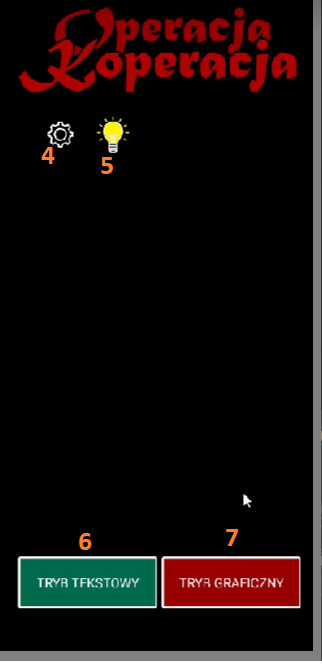
\includegraphics[width=8cm]{rys/opis3.png}
		\caption{Menu Główne v2}
		\label{rys:rysunek001}
	\end{center}
\end{figure}


\begin{enumerate}
	\setcounter{enumi}{3}
	\item Przycisk pozwalający nam przejść do ustawień, 
	\item Przycisk pozwalający nam przejść do poprzedniego menu głównego,
	\item Przycisk ten pozwala nam wybrać tryb tekstowy jako nasz tryb gry,
	\item Przycisk ten pozwala nam wybrać tryb graficzny jako nasz tryb gry.
\end{enumerate}

\subsection{Tryb tekstowy}
Po wejściu w tryb teksotwy ukazuje nam się takie okno jak na rys 6.3. Tutaj wprowadzamy kod w odpowiednim miejscu, który pozwoli nam zobaczyć podpowiedzi do danej zagadki. Kod jest widoczny w trybie graficznym razem z opisem zagadki w~komunikacie przed rozpoczęciem próby rozwiązania zagadki.
	\begin{figure}[!htb]
	\begin{center}
		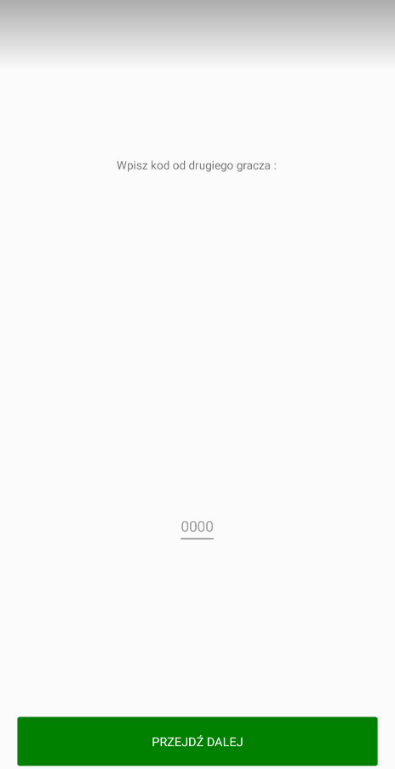
\includegraphics[width=8cm]{rys/tekstowy0.png}
		\caption{Tryb tekstowy}
		\label{rys:rysunek001}
	\end{center}
\end{figure}

\subsection{Labirynt}
Po wybraniu graficznego trybu gry zostajemy przeniesieni do pierwszej zagadki, którą jest labirynt. Na początku dostajemy informacje o zagadce jak i kod do trybu tekstowego dla naszego partnera. Ta zagadka polega na doprowadzeniu postaci (pomarańczowego kwadratu) do wyjścia. Osoba w trybie graficznym widzi kilka wersji labiryntu i musi wybrać właściwy na podstawie informacji jakie dostanie od partnera, po czym musi poprowadzić osobę z trybu graficznego do wyjścia. Każde wejście w ściane kończy się utratą życia i zresetowaniem pozycji postaci.
\\
\\
\\
\\
	\begin{figure}[!htb]
	\begin{center}
		
\includegraphics[width=8cm]{rys/opis2.png}
		\caption{Komunikat (Labirynt)}
		\label{rys:rysunek001}
	\end{center}
\end{figure}

\begin{enumerate}
	\setcounter{enumi}{7}
	\item Przycisk pozwalający nam rozpocząć grę,
\end{enumerate}

	\begin{figure}[!htb]
	\begin{center}
		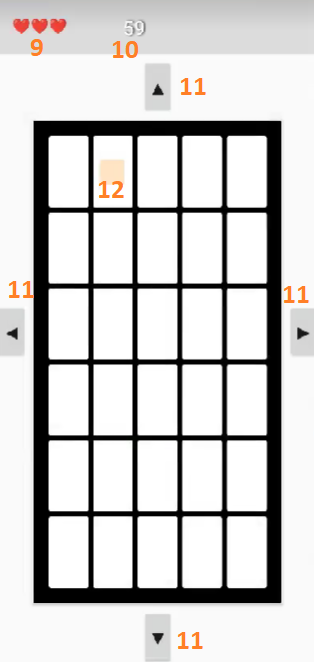
\includegraphics[width=8cm]{rys/opis4.png}
		\caption{Labirynt}
		\label{rys:rysunek001}
	\end{center}
\end{figure}

\begin{enumerate}
	\setcounter{enumi}{8}
	\item Licznik żyć (Zaczynamy mając 3 życia, w momencie utraty ostatniego przegrywamy),
	\item Timer (Pokazuje ile czasu mamy na daną zagadkę),
	\item Przyciski pozwalające poruszać naszą "postacią",
	\item Postać, którą sterujemy.
\end{enumerate}

	\begin{figure}[!htb]
	\begin{center}
		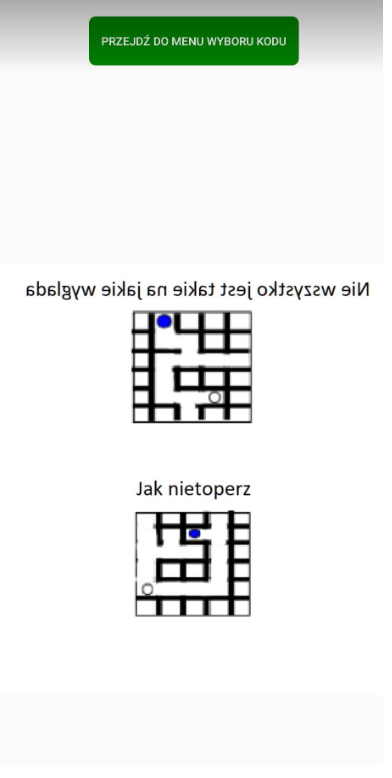
\includegraphics[width=8cm]{rys/tekstowy1.png}
		\caption{Tryb tekstowy (Labirynt)}
		\label{rys:rysunek001}
	\end{center}
\end{figure}
\hspace{-0.60cm}Jak widać na rys 6.6 tryb teksowy do zagadki "Labirynt"~ przedstawia możliwe rozłożenia labiryntu ale w tym trybie też są zagadki. Dla przykładu pierwsze rozłożenie labiryntu jest odbite lustrzanie od właściwego a drugie jest do góry nogami.
\subsection{Literaki}
Po przejściu "Labiryntu"~ zostajemy przeniesieni do kolejnej zagadki, którą są "Literaki". Podobnie jak w przypadku poprzedniej zagadki dostajemy opis tego co mamy zrobić i kod do trybu tekstowego. W tej zagadce chodzi o to, żeby razem z partnerem z trybu tektowego ustalić jakie hasło pozwoli nam przejść dalej. Gracz w trybie teksowym widzi dostępne słowa natomiast gracz w trybie graficznym musi za pomocą strzałek zmieniać litery na odpowiednich polach dopóki nie powstanie z nich jedno z tych słów. Liczba liter przypadająca na każde pole jest ograniczona.

	\begin{figure}[!htb]
	\begin{center}
		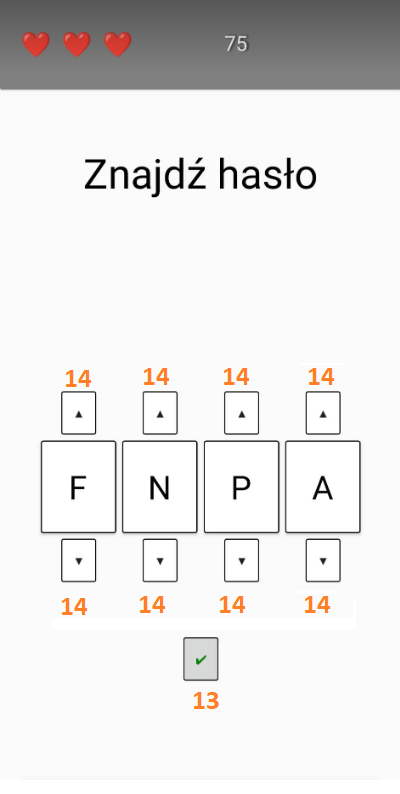
\includegraphics[width=8cm]{rys/opis6.png}
		\caption{Literaki}
		\label{rys:rysunek001}
	\end{center}
\end{figure}

\begin{enumerate}
	\setcounter{enumi}{12}
	\item Przycisk, którym zatwierdzamy hasło,
	\item Przyciski pozwalające na zmiane litery na odpowiednim miejscu.
\end{enumerate}

	\begin{figure}[!htb]
	\begin{center}
		
\includegraphics[width=8cm]{rys/opis8.png}
		\caption{Komunikat (Literaki))}
		\label{rys:rysunek001}
	\end{center}
\end{figure}

	\begin{figure}[!htb]
	\begin{center}
		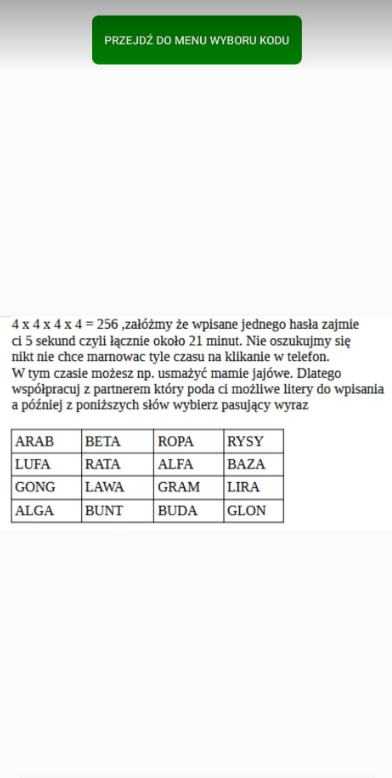
\includegraphics[width=8cm]{rys/tekstowy2.png}
		\caption{Tryb tekstowy (Literaki)}
		\label{rys:rysunek001}
	\end{center}
\end{figure}
\hspace{-0.60cm}Tryb tekstowy dla zagadki "Literaki" (rys 6.9) zawiera tabelę możliwych słow, autorski opis dlaczego nie warto próbować na siłę wpisywać hasła i dlaczego lepiej jest współpracować.
\\
\\
\\
\\
\\
\\
\\
\\
\\
\subsection{Kod Morsa}
Po ukończeniu "Literaków"~ zostajemy przeniesieni do zagadki, która nazywa się "Kod Morsa". Podobnie jak w przypadku poprzednich zagadek dostajemy opis zadań i kod do trybu tekstowego (rys 6.10). Ta zagadka jest podobna do ~"Literaków" z~ jedną różnicą. Gracz w tybie tekstowym ma opisane słowa za pomocą kodu morsa. Gracz trybu graficznego dostaje, poprzez włączanie i wyłącznie latarki, długie i~krótkie sygnały, które po skonsultowaniu z partnerem pozwolą odgadnąć hasło. 
\\
\\
	\begin{figure}[!htb]
	\begin{center}
		
\includegraphics[width=8cm]{rys/opis7.png}
		\caption{Komunikat (Kod Morsa)}
		\label{rys:rysunek001}
	\end{center}
\end{figure}
	\begin{figure}[!htb]
	\begin{center}
		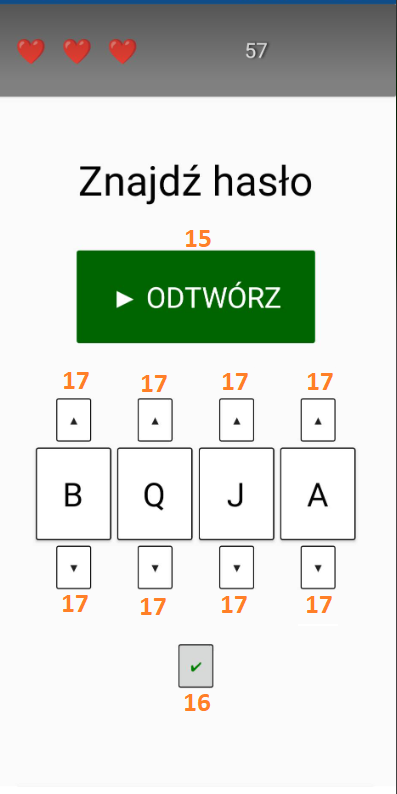
\includegraphics[width=8cm]{rys/opis5.png}
		\caption{Kod Morsa}
		\label{rys:rysunek001}
	\end{center}
\end{figure}

\begin{enumerate}
	\setcounter{enumi}{14}
	\item Przycisk, którym odtwarzamy kod morsa za pomocą latarki,
	\item Przycisk, którym zatwierdzamy hasło,
	\item Przyciski pozwalające na zmiane litery na odpowiednim miejscu.
	\\
	\\
	\\
	\\
	\\
	\\
\end{enumerate}

	\begin{figure}[!htb]
	\begin{center}
		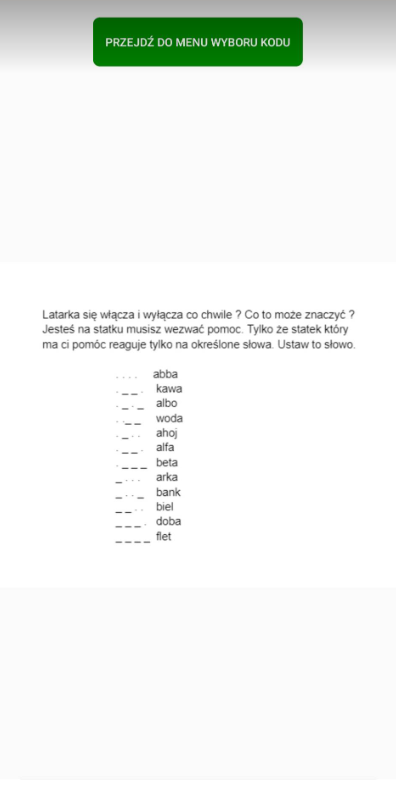
\includegraphics[width=8cm]{rys/tekstowy3.png}
		\caption{Tryb tekstowy (Kod Morsa)}
		\label{rys:rysunek001}
	\end{center}
\end{figure}
\hspace{-0.60cm}W trybie tekstowym (rys 6.12) dla trybu "Kod Morsa"~ są rozpisane słowa wraz z ich odpowiednikiem w kodzie. Kropka oznacza sygnał krótki a kreska sygnał długi.
\\
\\
\\
\\
\\
\subsection{Kolorki}
Po ukończeniu "Kodu Morsa"~ zostajemy przeniesieni do zagadki, która nazywa się "Kolorki". Podobnie jak w przypadku poprzednich zagadek dostajemy opis zadań i kod do trybu tekstowego (rys 6.13). Ta zagadka polega na odtworzeniu sygnału, który zostaje nam wyświetlony. W trybie tekstowym mamy opisane, przycisk w~jakim kolorze mamy nacisnąć po otrzymaniu konkretnego koloru. Gracz w trybie graficznym musi powtórzyć otrzymany kod. Początkowo jeden przycisk stopniowo zwiększając ich liczbę do pięciu.
\\
	\begin{figure}[!htb]
	\begin{center}
		
\includegraphics[width=8cm]{rys/opis9.png}
		\caption{Komunikat (Kolorki)}
		\label{rys:rysunek001}
	\end{center}
\end{figure}

	\begin{figure}[!htb]
	\begin{center}
		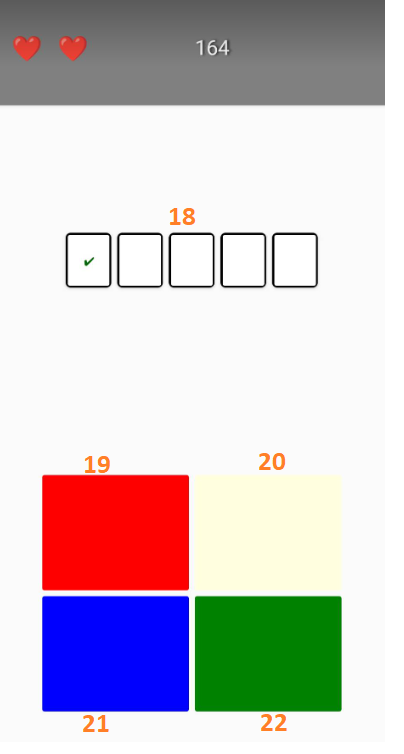
\includegraphics[width=8cm]{rys/opis10.png}
		\caption{Kolorki}
		\label{rys:rysunek001}
	\end{center}
\end{figure}

\begin{enumerate}
	\setcounter{enumi}{17}
	\item Licznik, który pokazuje ile jeszcze kolorów nam zostało do zgadnięcia,
	\item Przycisk, który odpowiada za określony kolor,
	\item Przycisk, który został wyróżniony i gracz musi kliknąć jego odpowiednik na podstawie informacji z trybu tekstowego,
	\item Przycisk, który odpowiada za określony kolor,
	\item Przycisk, który odpowiada za określony kolor.
	\\
	\\
\end{enumerate}

	\begin{figure}[!htb]
	\begin{center}
		
\includegraphics[width=8cm]{rys/tekstowy4.png}
		\caption{Tryb tekstowy (Kolorki)}
		\label{rys:rysunek001}
	\end{center}
\end{figure}
\hspace{-0.60cm}W trybie tekstowym dla tej zagadki (rys. 6.15) jest krótka historyjka i opis, który kolor ma kliknąć gracz w trybie graficznym jeżeli wyświetli się konkretny. Dla przykładu jeżeli gracz z trybu graficznego zobaczy wyróżniony zielony kolor musi wciisnąć czerwony przycisk
\\
\\
\\
\\
\\
\\
\subsection{Wielki Przycisk}
Po ukończeniu "Kolorków"~ zostajemy przeniesieni do zagadki, która nazywa się "Wielki Przycisk". Podobnie jak w przypadku poprzednich zagadek dostajemy opis zadań i kod do trybu tekstowego (rys 6.16). Ta zagadka polega na przytrzymaniu palca na przycisku przez określony czas zaczynając od określonego czasu na timerze. Wszysko zostało opisane w trybie tekstowym.
\\
\\
\\
\\
\\
	\begin{figure}[!htb]
	\begin{center}
		
\includegraphics[width=8cm]{rys/opis11.png}
		\caption{Komunikat (Wielki Przycisk)}
		\label{rys:rysunek001}
	\end{center}
\end{figure}
\begin{enumerate}
	\setcounter{enumi}{22}
	\item Wielki Przycisk, który mamy przytrzymać przez określoną liczbę sekund.
	\\
	\\
	\\
	\\
	\\
	\\
	\\
	\\
	\\
\end{enumerate}
	\begin{figure}[!htb]
	\begin{center}
		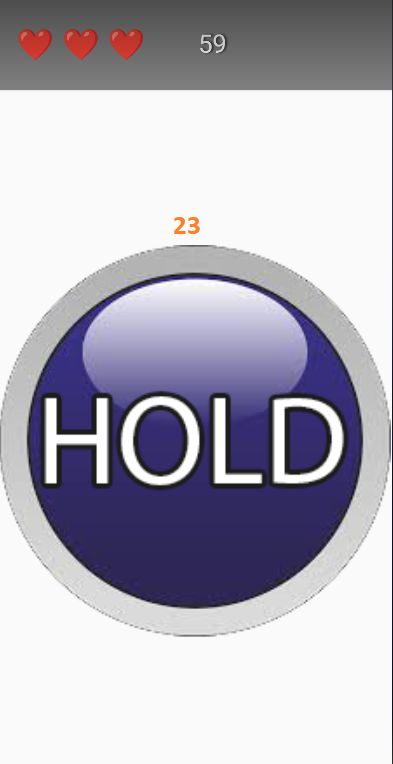
\includegraphics[width=8cm]{rys/opis12.png}
		\caption{Wielki Przycisk}
		\label{rys:rysunek001}
	\end{center}
\end{figure}

	\begin{figure}[!htb]
	\begin{center}
		
\includegraphics[width=8cm]{rys/tekstowy5.png}
		\caption{Tekstowy (Wielki Przycisk)}
		\label{rys:rysunek001}
	\end{center}
\end{figure}
\hspace{-0.60cm}W trybie tekstowym dla zagadki "Wielki Przycisk"~(rys 6.18) mamy napisane ile sekund i przy jakim czasie na timerze mamy przytrzymać przycisk.
\\
\\
\\
\\
\\
\\
\\
\\
\subsection{Tabela wyników}
Po przejściu wszyskich zagadek automatycznie przechodzimy do tabeli wyników i w odpowiednim polu wpisujemy swoje imie (rys 6.19). Po podaniu imienia nasz wynik zostaje dodany do tabeli wyników i zestawiony z innymi (rys 6.20).

	\begin{figure}[!htb]
	\begin{center}
		
\includegraphics[width=8cm]{rys/opis13.png}
		\caption{Tabela wyników (Podaj imie)}
		\label{rys:rysunek001}
	\end{center}
\end{figure}

	\begin{figure}[!htb]
	\begin{center}
		
\includegraphics[width=8cm]{rys/opis14.png}
		\caption{Tabela wyników}
		\label{rys:rysunek001}
	\end{center}
\end{figure}

       
%%%%%%%%%%%%%%%%%%% koniec treść główna dokumentu %%%%%%%%%%%%%%%%%%%%%
	\newpage
    \addcontentsline{toc}{section}{Literatura}  
	\printbibliography

    \newpage
    \hypersetup{linkcolor=black}
    \renewcommand{\cftparskip}{3pt}
    \clearpage
    \renewcommand{\cftloftitlefont}{\Large\bfseries\sffamily}
    \listoffigures
    \addcontentsline{toc}{section}{Spis rysunków}
	\thispagestyle{fancy}
	
    \newpage
    \renewcommand{\cftlottitlefont}{\Large\bfseries\sffamily}
    \def\listtablename{Spis tabel}
    \addcontentsline{toc}{section}{Spis tabel}\listoftables 
	\thispagestyle{fancy}
	
	\newpage
	\renewcommand{\cftlottitlefont}{\Large\bfseries\sffamily}
	\renewcommand\lstlistlistingname{Spis listingów}
	\addcontentsline{toc}{section}{Spis listingów}\lstlistoflistings 
	\thispagestyle{fancy}
	


    %lista rzeczy do zrobienia: wypisuje na koñcu dokumentu, patrz: pakiet todo.sty
    \todos
    %koniec listy rzeczy do zrobienia
\end{document}
